\begin{frame}
    \begin{center}
        \Huge ¡Bienvenidos!
    \end{center}
\end{frame}

\begin{frame}{Matrícula inicial}
    \begin{figure}
        \centering
        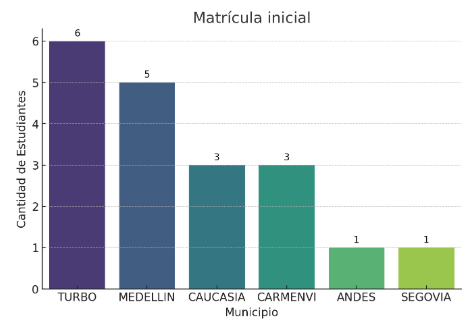
\includegraphics[width=0.8\linewidth]{figures/matricula-inicial.png}
    \end{figure}
\end{frame}

\begin{frame}{Generalidades}
    \begin{itemize}
        \item Horario de clases: martes y jueves 20:00 $-$ 22:00
        \item Clases en Zoom
        
        \begin{itemize}
            \item Enlace: {\color{blue}\url{udearroba.zoom.us/j/93686452220}}
            \item Meeting ID: 936 8645 2220
        \end{itemize} 
        \item Las sesiones se dividirán en:
        \begin{itemize}
            \item Teoría: aproximadamente una hora
            \item Práctica: aproximadamente 40 minutos
        \end{itemize}
        \item Horario de asesorías: martes 14:00 $-$ 15:00
        \begin{itemize}
            \item Virtual: {\color{blue}\url{meet.google.com/dgr-qdvk-qpr}}
            \item Presencial: sede Medellín Ciudad Universitaria, aula 6-120.
        \end{itemize}
        
    \end{itemize}
\end{frame}

\begin{frame}{Generalidades}
    \begin{itemize}
        \item Textos guía:
        \begin{itemize}
            \item Principal: Sears \& Zemansky (2013), \textit{Física Universitaria}. 13ava Ed., Vol. 1.
            \item Secundario: Serway \& Jewett (2008), \textit{Física para ciencias e ingeniería}. 7ma Ed., Vol. 1.
        \end{itemize}
        \item Esta presentación se actualizará clase a clase en los activos del repositorio {\color{blue}\url{github.com/diego-riosp/mechanics-202502}}.
    \end{itemize}
\end{frame}

\begin{frame}{Generalidades}
    Se propone que el tiempo de trabajo a la semana se divida de la siguiente forma:
\begin{itemize}
    \item 4 horas de sesiones de clase con el profesor
    \item 1 hora de lectura previa a la sesión de clase de las correspondientes sesiones.
    \item 1 hora de lectura posterior a la sesión de clase examinando los ejemplos del texto guía y enfatizando en los conceptos no comprendidos.
    \item 2 horas para el desarrollo de las preguntas y ejercicios planteados.
    \item 1 hora para leer materiales de apoyo, desarrollar las guías de estudio o realizar la autoevaluación en Ingeni@.
\end{itemize}
\end{frame}

\begin{frame}{Evaluación}
\begin{table}[]
    \centering
    \begin{tabular}{|c|c|c|c|c|}
    \hline
     \textbf{Examen} &  \textbf{Porcentaje (\%)}  &  \textbf{Fecha}& \textbf{Modalidad}\\\hline
     Quiz 1 & 5  &  04/09& Virtual\\\hline
     Parcial 1 & 20  &  09/09& Virtual\\\hline
     Quiz 2 & 5  & 09/10& Virtual \\\hline
     Parcial 2 & 20  & 11/10& Presencial\\\hline
     Quiz 3 & 5  & 11/11& Virtual\\\hline
     Parcial 3 (Oral) & 20 & 13/11& Virtual\\\hline
     Quiz 4 & 5  & 27/11& Virtual\\\hline
     Parcial 4 & 20  & 29/11& Presencial\\\hline
\end{tabular}
\end{table}

Los exámenes parciales 1 y 3 se realizarán en el horario de clase y en la fecha según la programación.

Los exámenes parciales 2 y 4 se realizarán en cada una de las sedes y seccionales según la programación, en el horario 14:00 $-$ 16:00.

\end{frame}

\begin{frame}
    \begin{center}
        \Huge ¿Preguntas?
    \end{center}
\end{frame}

\begin{frame}

    \begin{figure}
        \centering
        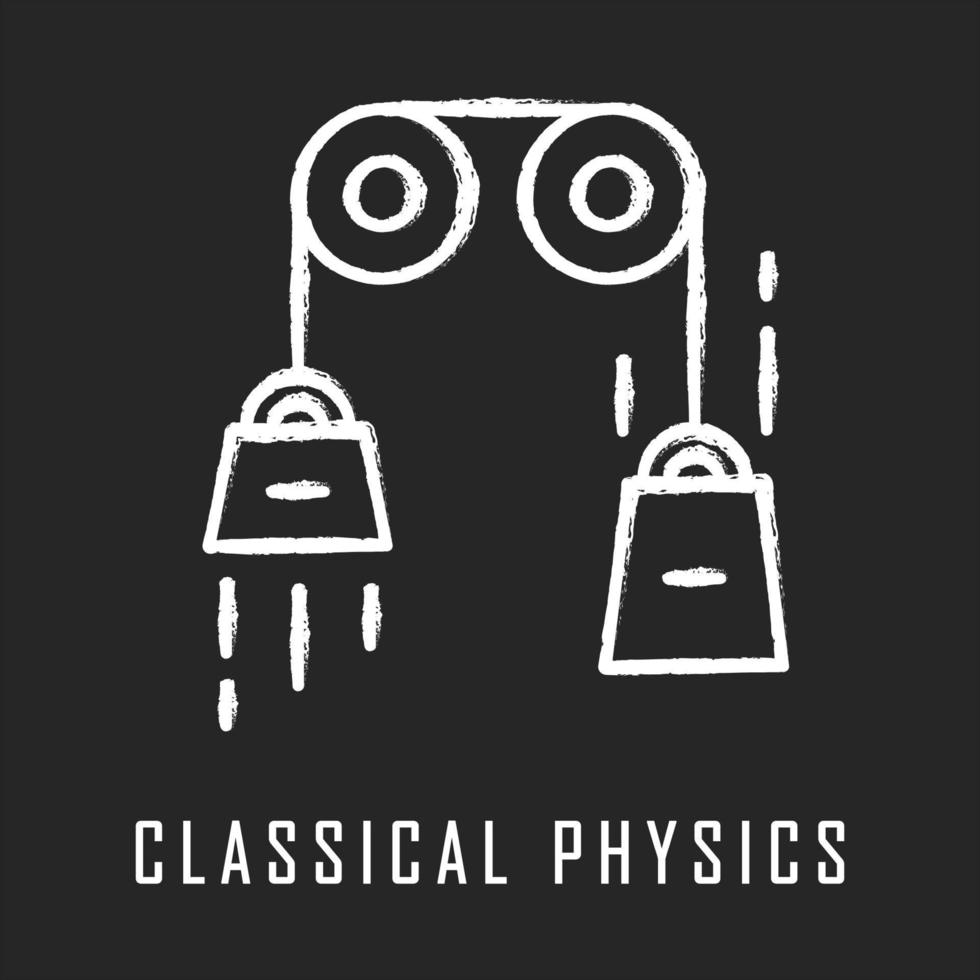
\includegraphics[width=0.5\linewidth]{figures/clasical-physics.jpg}
    \end{figure}
    
\begin{center}
    \LARGE Hagamos Física Clásica
\end{center}
    
\end{frame}

\begin{frame}
\begin{center}
    \Huge \textbf{Capítulo 1}
    
    \LARGE Unidades, cantidades físicas y vectores

    \textit{Comencemos desde el principio}
\end{center}
\end{frame}

\begin{frame}{Ideas}
    \begin{enumerate}
        \item La física es una ciencia experimental
        \item Un número empleado para describir cuantitativamente un fenómeno físico es una cantidad física
        \item Al medir una cantidad, siempre la \textit{comparamos} con un estándar de referencia. Si decimos que un Ferrari tiene una longitud de 4.53 m, queremos decir que es 4.53 veces más largo que una vara de cierto tamaño (1 m).
    \end{enumerate}
\end{frame}

\begin{frame}{¿Qué se compara al medir?}
    \begin{figure}
        \centering
        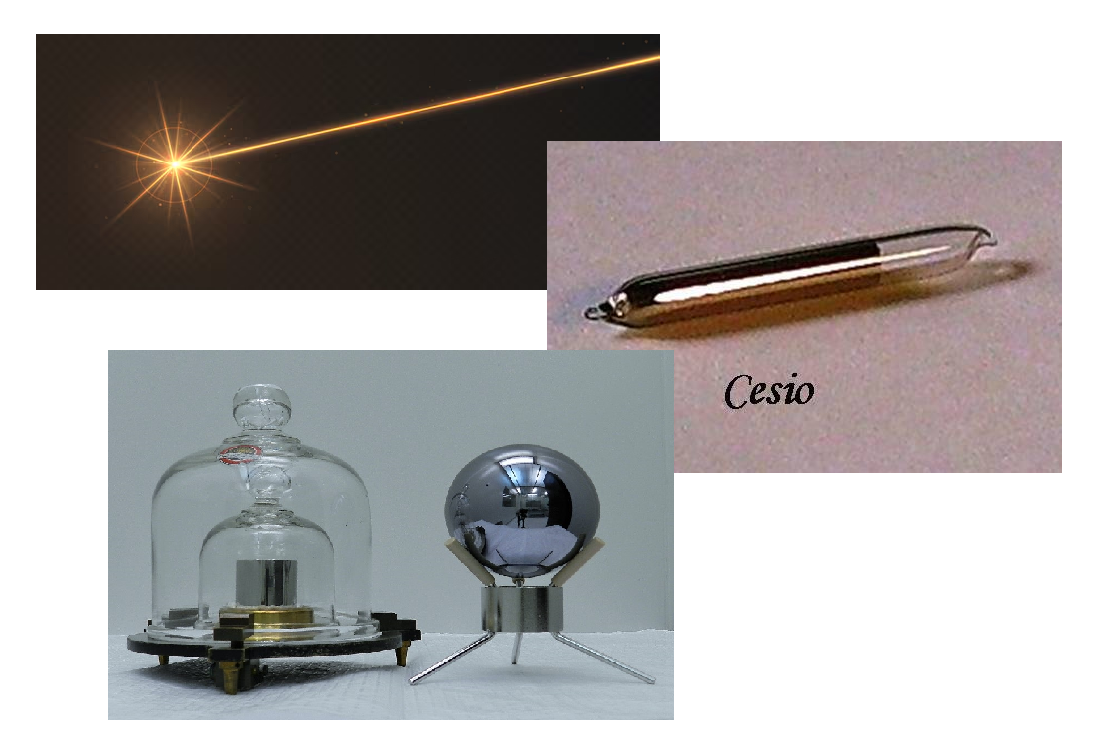
\includegraphics[width=0.8\linewidth]{figures/que-se-mide.png}
    \end{figure}

    Por ejemplo, para medir distancia, comparemos con la luz. Para medir masas, comparemos con objetos que nunca más volveremos a tocar. Para medir tiempo, comparemos con átomos.    
\end{frame}

\begin{frame}{¿Qué podemos medir?}

\textbf{Magnitud física}

    Una magnitud física es toda propiedad de un fenómeno, cuerpo o sustancia que se puede medir y expresar con un número y una unidad.
    
    \vspace{1em}

    \begin{columns}
        \column{0.45\textwidth}
        \textbf{Fundamentales}
        
        Se definen por sí mismas
        \begin{itemize}
            \item Tiempo
            \item Longitud
            \item Masa
            \item Temperatura
            \item Cantidad de sustancia
            \item Intensidad luminosa
            \item Carga eléctrica
        \end{itemize}
        $$\vdots$$
        
        \column{0.45\textwidth}
        \textbf{Derivadas}
        
        Se obtienen a partir de las fundamentales
        \begin{itemize}
            \item Velocidad
            \item Aceleración
            \item Fuerza
            \item Potencia
            \item Energía
            \item Corriente eléctrica
        \end{itemize}
        $$\vdots$$
    \end{columns}
\end{frame}

\begin{frame}{¿Qué referencias usamos para medir?}
\textbf{Unidades de medida}

Las unidades de medida son estándares o referencias que se usan para expresar el valor de una magnitud física.

\vspace{1em}

\textit{Ejemplos:} metros, pulgadas, yardas, segundos, eones, años, gramos, coulombs, newtons, amperios, voltios, celcius, parsec, años luz, candelas, etc.

\end{frame}

\begin{frame}{¿Qué estándares usamos para medir?}
    \textbf{Sistemas de medida}

Un sistema de medida es un conjunto organizado de unidades de medida y reglas que se usan para medir y expresar magnitudes físicas de forma uniforme.

Es como un “idioma común” para las mediciones: define qué unidades usar y cómo relacionarlas.

    \begin{table}[h]
\centering
\caption{Unidades base del Sistema Internacional (SI)}
\begin{tabular}{|l|l|l|}
\hline
\textbf{Magnitud} & \textbf{Unidad} & \textbf{Símbolo} \\ \hline
Longitud & metro & m \\ \hline
Masa & kilogramo & kg \\ \hline
Tiempo & segundo & s \\ \hline
Temperatura & kelvin & K \\ \hline
Corriente eléctrica & amperio & A \\ \hline
Cantidad de sustancia & mol & mol \\ \hline
Intensidad luminosa & candela & cd \\ \hline
\end{tabular}
\end{table}
\end{frame}

\begin{frame}
    \begin{table}[h]
\centering
\caption{Unidades comunes en el sistema inglés}
\begin{tabular}{|l|l|l|}
\hline
\textbf{Magnitud} & \textbf{Unidad} & \textbf{Símbolo} \\ \hline
Longitud & pie & ft \\ \hline
Longitud & pulgada & in \\ \hline
Masa & libra & lb \\ \hline
Tiempo & segundo & s \\ \hline
Temperatura & grado Fahrenheit & $^\circ$F \\ \hline
Fuerza & libra-fuerza & lbf \\ \hline
Velocidad & milla por hora & mph \\ \hline
\end{tabular}
\end{table}

\end{frame}

\begin{frame}{Equivalencias entre sistemas}
\footnotesize
    \begin{table}[h]
\centering
\caption{Equivalencias entre el Sistema Internacional y el Sistema Inglés}
\begin{tabular}{|l|l|l|}
\hline
\textbf{Magnitud} & \textbf{Sistema Internacional (SI)} & \textbf{Sistema Inglés} \\ \hline
Longitud & 1 metro (m) = 3.2808 pies (ft) & 1 pie (ft) = 0.3048 m \\ \hline
Longitud & 1 kilómetro (km) = 0.6214 millas (mi) & 1 milla (mi) = 1.6093 km \\ \hline
Masa & 1 kilogramo (kg) = 2.2046 libras (lb) & 1 libra (lb) = 0.4536 kg \\ \hline
Fuerza & 1 newton (N) = 0.2248 libras-fuerza (lbf) & 1 lbf = 4.4482 N \\ \hline
Velocidad & 1 m/s = 2.2369 millas/hora (mph) & 1 mph = 0.4470 m/s \\ \hline
Temperatura & $^\circ$C = ($^\circ$F - 32) × 5/9 & $^\circ$F = ($^\circ$C × 9/5) + 32 \\ \hline
\end{tabular}
\end{table}

\end{frame}

\begin{frame}{Ejemplos}

\textbf{Ejemplo 1: Inglés $\rightarrow$ SI}  

Convertir \SI{12}{\foot} a metros:

\[
\SI{12}{\foot} \times \frac{\SI{0.3048}{\metre}}{\SI{1}{\foot}} 
= \SI{3.6576}{\metre}
\]

\textbf{Ejemplo 2: SI $\rightarrow$ Inglés}  

Convertir \SI{5}{\metre} a pies:

\[
\SI{5}{\metre} \times \frac{\SI{3.2808}{\foot}}{\SI{1}{\metre}} 
= \SI{16.404}{\foot}
\]
\end{frame}

\begin{frame}{¿Cómo evitamos números muy largos?}

\textbf{Prefijos}

    Los prefijos son partículas que se colocan delante del nombre o símbolo de una unidad para indicar que la magnitud medida es un múltiplo o un submúltiplo de esa unidad.

En otras palabras, los prefijos nos ahorran escribir muchos ceros, tanto a la izquierda como a la derecha de la coma decimal.
\end{frame}

\begin{frame}

\footnotesize

    \begin{table}[h]
\centering
\begin{tabular}{|l|l|l|}
\hline
\textbf{Prefijo} & \textbf{Símbolo} & \textbf{Factor de multiplicación} \\ \hline
yotta  & Y  & $10^{24}$  \\ \hline
zetta  & Z  & $10^{21}$  \\ \hline
exa    & E  & $10^{18}$  \\ \hline
peta   & P  & $10^{15}$  \\ \hline
tera   & T  & $10^{12}$  \\ \hline
giga   & G  & $10^{9}$   \\ \hline
mega   & M  & $10^{6}$   \\ \hline
kilo   & k  & $10^{3}$   \\ \hline
hecto  & h  & $10^{2}$   \\ \hline
deca   & da & $10^{1}$   \\ \hline
—      & —  & $10^{0}$   \\ \hline
deci   & d  & $10^{-1}$  \\ \hline
centi  & c  & $10^{-2}$  \\ \hline
milli  & m  & $10^{-3}$  \\ \hline
micro  & $\mu$ & $10^{-6}$  \\ \hline
nano   & n  & $10^{-9}$  \\ \hline
pico   & p  & $10^{-12}$ \\ \hline
femto  & f  & $10^{-15}$ \\ \hline
atto   & a  & $10^{-18}$ \\ \hline
zepto  & z  & $10^{-21}$ \\ \hline
yocto  & y  & $10^{-24}$ \\ \hline
\end{tabular}
\end{table}
\end{frame}

\begin{frame}{Ejemplos}
    \begin{itemize}
    \item \SI{1}{\kilo\metre} $\;=\;$ 1000 metros $\;=\;$ $10^{3} \ \si{\metre}$
    \item \SI{1}{\milli\metre} $\;=\;$ 0.001 metros $\;=\;$ $10^{-3} \ \si{\metre}$
    \item \SI{1}{\micro\second} $\;=\;$ 0.000001 segundos $\;=\;$ $10^{-6} \ \si{\second}$
\end{itemize}
\end{frame}

\begin{frame}
    \begin{center}
        \Huge ¿Preguntas?
    \end{center}
\end{frame}

\begin{frame}
    Para resolver los ejercicios que a continuación se presentan, implemente las siguientes equivalencias.

    \begin{align}
        \num{1}\,\unit{in} &= \num{2.54}\,\unit{cm}\\
        \num{1}\,\unit{ft} &= \num{30.48}\,\unit{cm}\\
        \num{1}\,\unit{yd} &= \num{0.91}\,\unit{m}\\
        \num{1}\,\unit{mi} &= \num{1.609}\,\unit{km}\\
        \num{1}\,\unit{lb} &= \num{453.59}\,\unit{g}\\
        \num{1}\,\unit{fl oz} &= \num{29.57}\,\unit{ml}\\
        \num{1}\,\unit{ton} &= \num{907.19}\,\unit{kg}\\
        \num{1}\,\unit{oz} &= \num{28.35}\,\unit{kg}\\
        \num{1}\,\unit{gal} &= \num{3.79}\,\unit{l}
    \end{align}
\end{frame}

\begin{frame}{Ejercicios propuestos}
    \begin{multicols}{3}
    \begin{enumerate}
    \item $\num{15} \,\unit{in}\rightarrow\unit{cm}$
    \item $\num{3.5} \,\unit{ft}\rightarrow\unit{cm}$
    \item $\num{2.1} \,\unit{yd}\rightarrow\unit{in}$
    \item $\num{12} \,\unit{mi}\rightarrow\unit{cm}$
    \item $\num{450} \,\unit{lb}\rightarrow\unit{ton}$
    \item $\num{8} \,\unit{lb}\rightarrow\unit{g}$
    \item $\num{56} \,\unit{oz}\rightarrow\unit{g}$
    \item $\num{10} \,\unit{gal}\rightarrow\unit{l}$
    \item $\num{5} \,\unit{m}\rightarrow\unit{in}$
    \item $\num{1.8} \,\unit{cm}\rightarrow\unit{ft}$
    \item $\num{3.2} \,\unit{m}\rightarrow\unit{yd}$
    \item $\num{25} \,\unit{km}\rightarrow\unit{mi}$
    \item $\num{0.75} \,\unit{ton}\rightarrow\unit{kg}$
    \item $\num{500} \,\unit{g}\rightarrow\unit{oz}$
    \item $\num{100} \,\unit{g}\rightarrow\unit{lb}$
    \item $\num{20} \,\unit{l}\rightarrow\unit{gal}$
    \item $\num{48} \,\unit{in}\rightarrow\unit{cm}$
    \item $\num{7} \,\unit{ft}\rightarrow\unit{cm}$
    \item $\num{6} \,\unit{yd}\rightarrow\unit{m}$
    \item $\num{35} \,\unit{mi}\rightarrow\unit{km}$
    \item $\num{2} \,\unit{ton}\rightarrow\unit{kg}$
    \item $\num{2.5} \,\unit{lb}\rightarrow\unit{g}$
    \item $\num{5} \,\unit{oz}\rightarrow\unit{g}$
    \item $\num{15} \,\unit{gal}\rightarrow\unit{l}$
    \item $\num{2.4} \,\unit{cm}\rightarrow\unit{ft}$
    \item $\num{8} \,\unit{m}\rightarrow\unit{yd}$
    \item $\num{36} \,\unit{in}\rightarrow\unit{ft}$
    \item $\num{5.5} \,\unit{ft}\rightarrow\unit{yd}$
    \item $\num{12} \,\unit{yd}\rightarrow\unit{mi}$
    \item $\num{5280} \,\unit{ft}\rightarrow\unit{mi}$
    \item $\num{96} \,\unit{oz}\rightarrow\unit{lb}$
    \item $\num{120} \,\unit{lb}\rightarrow\unit{ton}$
    \item $\num{0.75} \,\unit{ton}\rightarrow\unit{lb}$
    \item $\num{256} \,\unit{oz}\rightarrow\unit{ton}$
    \item $\num{192} \,\unit{fl\,oz}\rightarrow\unit{gal}$
    \item $\num{144} \,\unit{in^2}\rightarrow\unit{ft^2}$
    \item $\num{9} \,\unit{ft^2}\rightarrow\unit{yd^2}$
    \item $\num{27} \,\unit{ft^3}\rightarrow\unit{yd^3}$
    \item $\num{1728} \,\unit{in^3}\rightarrow\unit{ft^3}$
    \item $\num{1760} \,\unit{yd}\rightarrow\unit{mi}$
    \item $\num{2.5} \,\unit{mi}\rightarrow\unit{yd}$
    \end{enumerate}
\end{multicols}
\end{frame}

\begin{frame}
\setlength{\columnsep}{0.5cm} %
\footnotesize
    \begin{multicols}{2}
    \begin{enumerate}
    \item $\num{6728.73004} \,\unit{km}\rightarrow\unit{dm}$
    \item $\num{7526859842.59} \,\unit{mg}\rightarrow\unit{hg}$
    \item $\num{0.000000598} \,\unit{\mu s}\rightarrow\unit{fs}$
    \item $\num{59863.254701} \,\unit{Glb}\rightarrow\unit{Mlb}$
    \item $\num{2.0000256} \,\unit{Ymol}\rightarrow\unit{Tmol}$
    \item $\num{0.0000000000000001} \,\unit{Tm}\rightarrow\unit{nm}$
    \item $\num{100000000000000000} \,\unit{cm}\rightarrow\unit{Zm}$
    \item $\num{0.000236589725} \,\unit{hs}\rightarrow\unit{ps}$
    \item $\num{0.0002555} \,\unit{cm}\rightarrow\unit{dam}$
    \item $\num{560029698.2256301} \,\unit{kb}\rightarrow\unit{Gb}$
    \item $\num{1} \,\unit{Y^\circ C}\rightarrow\unit{y^\circ C}$
    \item $\num{0.00000003265871} \,\unit{\mu K}\rightarrow\unit{kK}$
    \item $\num{5897.003} \,\unit{mL}\rightarrow\unit{L}$
    \item $\num{0.00001254} \,\unit{Gm}\rightarrow\unit{km}$
    \item $\num{9547863.25} \,\unit{cm^3}\rightarrow\unit{m^3}$
    \item $\num{0.000000025} \,\unit{Pb}\rightarrow\unit{Tb}$
    \item $\num{325.698} \,\unit{g}\rightarrow\unit{mg}$
    \item $\num{0.00002536} \,\unit{ds}\rightarrow\unit{ms}$
    \item $\num{95872365.4} \,\unit{dm^2}\rightarrow\unit{km^2}$
    \item $\num{0.0000000000147} \,\unit{Ts}\rightarrow\unit{Gs}$
    \item $\num{1.254} \,\unit{pm}\rightarrow\unit{fm}$
    \item $\num{325.698} \,\unit{hl}\rightarrow\unit{ml}$
    \item $\num{9587.002} \,\unit{km}\rightarrow\unit{m}$
    \item $\num{0.000000000000365} \,\unit{Ms}\rightarrow\unit{ns}$
    \item $\num{123.589} \,\unit{fl}\rightarrow\unit{pl}$
    \item $\num{0.53248} \,\unit{kb^2}\rightarrow\unit{db^2}$
\end{enumerate}
\end{multicols}
\end{frame}

\begin{frame}{Incertidumbre}
    Toda medición tiene incertidumbre, la cual depende del instrumento y la técnica utilizada.

\vspace{1em}
    
\textbf{Un ejemplo:} medir con una regla común da un espesor de 3 mm con una precisión solo al milímetro más cercano, mientras que un micrómetro da 2.91 mm con precisión al 0.01 mm.

\vspace{1em}

\textit{La medición con menor incertidumbre es más exacta}.
\end{frame}

\begin{frame}{Cifras significativas}
    Las \textbf{cifras significativas} son los dígitos de una medición que aportan 
información real sobre su valor, es decir, aquellos que se conocen con certeza 
más el primer dígito incierto.

\vspace{1em}

Sirven para \textbf{indicar la precisión} de una medición y dependen tanto del 
instrumento usado como de la forma de registrar el dato.
\end{frame}

\begin{frame}
    \textbf{Reglas básicas para identificarlas}
\begin{enumerate}
    \item \textbf{Todos los dígitos distintos de cero} son significativos.  
    Ej.: $345$ $\rightarrow$ 3 cifras significativas.
    
    \item \textbf{Los ceros entre dígitos distintos de cero} son significativos.  
    Ej.: $2007$ $\rightarrow$ 4 cifras significativas.
    
    \item \textbf{Los ceros a la izquierda} no son significativos 
    (solo indican posición decimal).  
    Ej.: $0.0045$ $\rightarrow$ 2 cifras significativas.
    
    \item \textbf{Los ceros a la derecha} son significativos si hay punto decimal.  
    Ej.: $45.00$ $\rightarrow$ 4 cifras significativas.
    
    \item En notación científica, todos los dígitos del número principal son 
    significativos.  
    Ej.: $6.020 \times 10^{23}$ $\rightarrow$ 4 cifras significativas.
\end{enumerate}
\end{frame}

\begin{frame}
    \textbf{Ejemplo:} Si se mide una longitud como $12.34 \ \text{cm}$, las cuatro 
cifras indican precisión hasta la centésima de centímetro; el último dígito (4) 
es incierto, pero forma parte de la información significativa.
\end{frame}

\begin{frame}{Aproximaciones}
    A continuación se muestra la diferencia entre aproximar un número 
por \textbf{truncamiento} y por \textbf{redondeo} a diferentes cifras decimales.

\begin{center}
\begin{tabular}{cccc}
\toprule
\textbf{Valor original} & \textbf{Cifras decimales} & \textbf{Truncamiento} & \textbf{Redondeo} \\
\midrule
$3.14159$ & 4 & $3.1415$ & $3.1416$ \\
$3.14159$ & 3 & $3.141$  & $3.142$  \\
$3.14159$ & 2 & $3.14$   & $3.14$   \\
$3.14159$ & 1 & $3.1$    & $3.1$    \\
$3.14159$ & 0 & $3$      & $3$      \\
\bottomrule
\end{tabular}
\end{center}

\textbf{Explicación:}
\begin{itemize}
    \item En el \textbf{truncamiento} se cortan los dígitos después de la cifra deseada sin considerar su valor.
    \item En el \textbf{redondeo} se aumenta en una unidad la última cifra conservada si el siguiente dígito es 5 o mayor.
\end{itemize}
\end{frame}

\begin{frame}
\begin{center}
    \Huge ¿Preguntas?
\end{center}
\end{frame}

\begin{frame}
    \begin{figure}
        \centering
        
\includegraphics[width=0.8\linewidth]{figures/meme-1.jpeg}
    \end{figure}
\end{frame}

\begin{frame}{Ejercicios propuestos}
\footnotesize
    \begin{table}[H]
    \centering
    \begin{tabular}{|c|c|M{1cm}|M{1cm}|M{1cm}|M{1cm}|}
    \hline
        Literal & Cantidad & Sin prefijo & Notación científica & Aprox. & Prefijo  \\\hline\hline
        A & $\num{7128433.076} \,\unit{km}$ & & &  & \\\hline
        B & $\num{0.00000003071} \,\unit{b}$ & & &  & \\\hline
        C & $\num{0.002716} \,\unit{mA}$ & & &  & \\\hline
        D & $\num{24182.33708} \,\unit{\mu^\circ C}$ & & &  & \\\hline
        E & $\num{88807166254} \,\unit{hb}$ & & &  & \\\hline
        F & $\num{0.0000300008} \,\unit{m}$ & & &  & \\\hline
        G & $\num{3821714321.66} \,\unit{pJ}$ & & &  & \\\hline
        H & $\num{6082417.9127} \,\unit{cl}$ & & &  & \\\hline
        I & $\num{0.0000000000001} \,\unit{Tg}$ & & &  & \\\hline
        J & $\num{421809718.006} \,\unit{cg}$ & & &  & \\\hline
        K & $\num{0.0000070128002} \,\unit{s}$ & & &  & \\\hline
        L & $\num{1111111100.20001} \,\unit{K}$ & & &  & \\\hline
    \end{tabular}
\end{table}
\end{frame}

\begin{frame}
\footnotesize
    \begin{table}[H]
    \centering
    \begin{tabular}{|c|c|M{1cm}|M{1cm}|M{1cm}|M{1cm}|}
    \hline
        Literal & Cantidad & Sin prefijo & Notación científica & Aprox. & Prefijo  \\\hline\hline
        M & $\num{0.000000000000000007} \,\unit{Pb}$ & & &  & \\\hline
        N & $\num{28421571.00382} \,\unit{\mu K}$ & & &  & \\\hline
        O & $\num{222341567.886} \,\unit{ms}$ & & &  & \\\hline
        P & $\num{718718210047216687} \,\unit{fs}$ & &  &  & \\\hline
        Q & $\num{800000000000000} \,\unit{g}$ & & &  & \\\hline
        R & $\num{330182.43} \,\unit{km}$ & & &  & \\\hline
        S & $\num{1050000233} \,\unit{b}$ & & &  & \\\hline
        T & $\num{0.0000000001} \,\unit{cm}$ & & &  & \\\hline
        U & $\num{323998417992.0006} \,\unit{m}$ & & &  & \\\hline
        V & $\num{8240017.83} \,\unit{cb}$ & & &  & \\\hline
        W & $\num{11717111111.17} \,\unit{\mu C}$ & & &  & \\\hline
        X & $\num{9999999999999} \,\unit{m}$ & & &  & \\\hline
        Y & $\num{2130000000} \,\unit{ml}$ & & &  & \\\hline
        Z & $\num{0.00000000082} \,\unit{GA}$ & & &  & \\\hline
    \end{tabular}
\end{table}
\end{frame}

\begin{frame}
\begin{center}
    {\Huge \textbf{VECTORES}}

    \vspace{1em}
    
    (¡ojo, que está en mayúscula!)
\end{center}
    
\end{frame}

\begin{frame}
    
    \begin{center}
    Sin rodeos:
    
    \vspace{2em}
    
        \LARGE \textbf{UN VECTOR ES UN NÚMERO DE VARIAS DIMENSIONES.}
    \end{center}
    
\end{frame}

\begin{frame}

\begin{center}
    \Huge FIN.
\end{center}

\end{frame}

\begin{frame}{¿Por qué vectores?}
    Algunas magnitudes físicas, como tiempo, temperatura, masa o densidad, se describen solo con un número y una unidad (cantidades \textit{escalares}). Sin embargo, otras, como el desplazamiento, la velocidad o la fuerza, requieren también una dirección para estar completamente definidas. Estas magnitudes con módulo y dirección se llaman \textit{vectoriales}.
\end{frame}

\begin{frame}{Tipos de magnitudes físicas}
    \begin{center}
\begin{tabular}{ll}
\toprule
\textbf{Escalares} & \textbf{Vectoriales} \\
\midrule
Tiempo          & Desplazamiento \\
Temperatura     & Velocidad \\
Masa            & Aceleración \\
Densidad        & Fuerza \\
Energía         & Momento lineal \\
Presión         & Campo eléctrico \\
Trabajo         & Campo magnético \\
Potencia        & Impulso \\
$$\vdots$$        & $$\vdots$$ \\
\bottomrule
\end{tabular}
\end{center}
\end{frame}

\begin{frame}{Ejercicios}
    Descomponga rectangularmente los siguientes vectores 
    
    \begin{multicols}{2}
        
        \begin{figure}[H]
            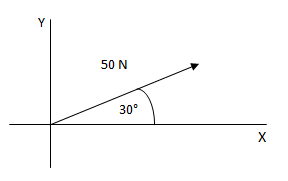
\includegraphics[width=0.4\textwidth]{figures/composicion-y-descomposicion-1.jpg}
        \end{figure}
        
        
        \begin{figure}[H]
            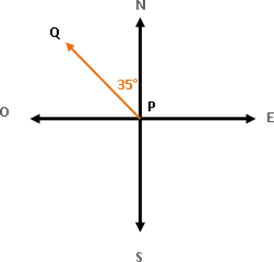
\includegraphics[width=0.4\textwidth]{figures/suma2.jpg}
        \end{figure}
        
        $$Q = 100 \text{ N}$$
        
    \end{multicols}
\end{frame}

\begin{frame}
\begin{center}
    \Large Vayamos al tablero para ver cómo funciona.
    \begin{figure}
    \centering
    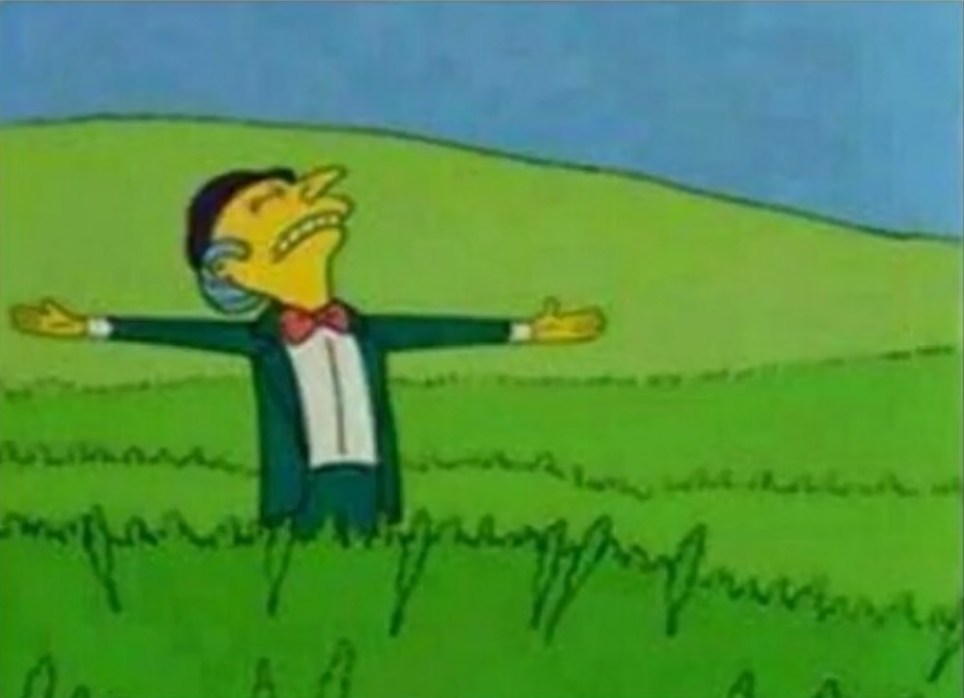
\includegraphics[width=0.6\linewidth]{figures/imagen1.png}
\end{figure}
\end{center}
\end{frame}

\begin{frame}
    Se dice que un sistema est\'a en equilibrio traslacional si $\vec{F}_N = \vec{0}$. Discrimine el estado de equilibrio de los siguientes sistemas en los cuales actúan las fuerzas dadas.
    
    \begin{itemize}
        \item[a)] $\vec{F}_1 = (1000 \text{ N} , 37^\circ)$ y $\vec{F}_2 = (1000 \text{ N} , 217^\circ)$.
        \item[b)] $\vec{F}_1 = (1000 \text{ N} , 270^\circ)$ y $\vec{F}_2 = (800 \text{ N} , 90^\circ)$.
        \item[c)] $\vec{F}_1 = (440 \text{ N} , 225^\circ)$ y $\vec{F}_2 = (440 \text{ N} , 315^\circ)$.
        \item[d)] $\vec{F}_1 = (800 \text{ N} , 0^\circ)$ y $\vec{F}_2 = (800 \text{ N} , 180^\circ)$.
    \end{itemize}
\end{frame}

    \begin{frame}
    \begin{multicols}{2}
    \begin{figure}[H]
            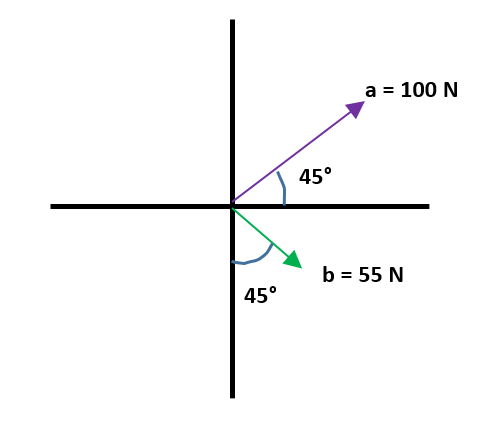
\includegraphics[width=0.5\textwidth]{figures/Ejercicios-de-suma-de-vectores-1.png}
        \end{figure}
        
        \begin{figure}[H]
        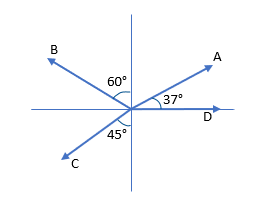
\includegraphics[width=0.5\textwidth]{figures/vectores-30.png}
        \end{figure}
        
        $A = 40 \text{ N}$, $B = 75 \text{ N}$, $C = 50 \text{ N}$ y $D = 45 \text{ N}$.
\end{multicols}
        
    \end{frame}

\begin{frame}
\begin{center}
    \Huge \textbf{Capítulos 2 y 3}
    
    \LARGE Cinemática

    \textit{La descripción matemática del movimiento}
\end{center}
    
\end{frame}

\begin{frame}
    \begin{center}
        {\LARGE ¿Qué es la cinemática?}

        \vspace{2em}

        \textbf{En la siguiente diapositiva lo explico contundentemente.}
    \end{center}

    
\end{frame}

\begin{frame}
    \begin{figure}
    \centering
    
\includegraphics[width=0.8\linewidth]{figures/meme2.jpeg}
\end{figure}
\end{frame}

\begin{frame}{Cinemática}
    En otras palabras...

    \vspace{1em}
    
    \begin{center}
        \textit{Estudia el movimiento de los cuerpos sin considerar las causas que lo producen.}
    \end{center}
    

    \vspace{1em}

    \textbf{Qué estudia:} el movimiento.

\textbf{Qué ignora:} las causas del movimiento (eso lo hace la dinámica).

\textbf{Magnitudes clave:} posición, desplazamiento, velocidad, aceleración, tiempo.
    
\end{frame}

\begin{frame}{Variables cinemáticas}
Las magnitudes físicas imperativas en la cinemática son las siguientes.

    \begin{itemize}
        \item \textbf{Tiempo:} magnitud fundamental que permite ordenar la secuencia de los sucesos (pasado, presente, futuro), medir la duración y la separación entre acontecimientos, y determinar su simultaneidad. Típicamente se denota con la letra $t$.
    \end{itemize}
\end{frame}

\begin{frame}
    \begin{itemize}
        \item \textbf{Posición:} Ubicación de un objeto en el espacio, relativo a un punto de referencia. Se mide en unidades de longitud. Típicamente se denota con la letra $x$ y, en general, es una función del tiempo $x=x(t)$.
        \item \textbf{Desplazamiento:} Cambio en la posición de un objeto: $$\Delta x = x(t_\text{final})-x(t_\text{inicial}).$$ Se mide en unidades de longitud.
        \item \textbf{Distancia:} Suma de los valores absolutos de los desplazamientos de un objeto. Típicamente se denota con la letra $d$. Está dada por $$d = \sum_{n=1}^N\lvert\Delta x\lvert_n.$$
    \end{itemize}
\end{frame}

\begin{frame}{Concepto de velocidad}
    Considerar una partícula que recorre espacios iguales en tiempos iguales. Es decir, su posición respecto de un punto de referencia se incrementa de forma directamente proporcional al tiempo.

    \begin{figure}
        \centering
        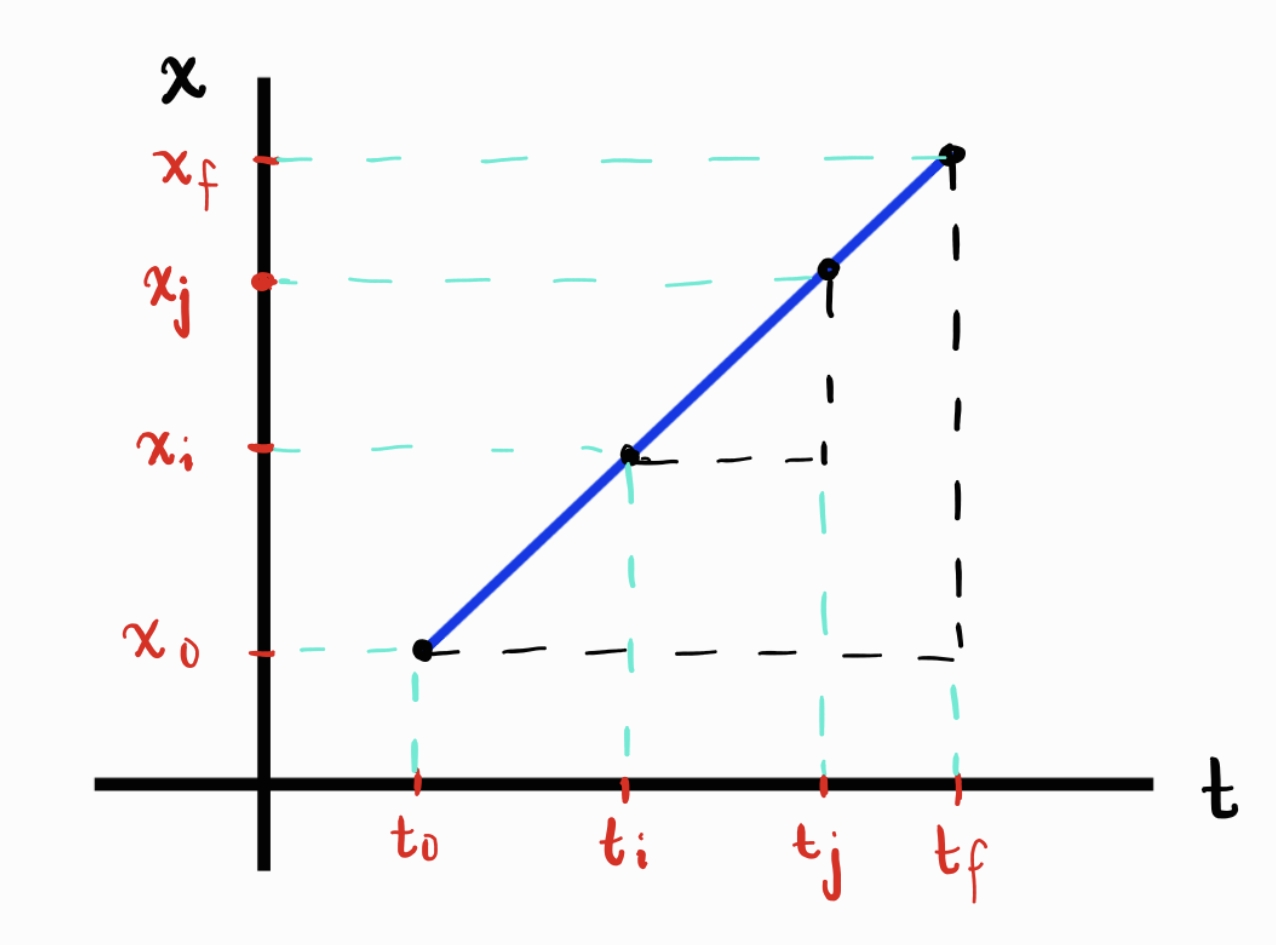
\includegraphics[width=0.4\linewidth]{figures/XvsT1.jpg}
    \end{figure}

    En esta situación, la \textbf{velocidad} se define como la variación de la posición respecto de la variación en el tiempo dentro de los mismos intervalos, es decir, $$v=\frac{x_f-x_0}{t_f-t_0}=\frac{x_j-x_i}{t_j-t_i}=\frac{\Delta x}{\Delta t}.$$
    
\end{frame}

\begin{frame}{Velocidad instantanea}

    \begin{figure}
        \centering
        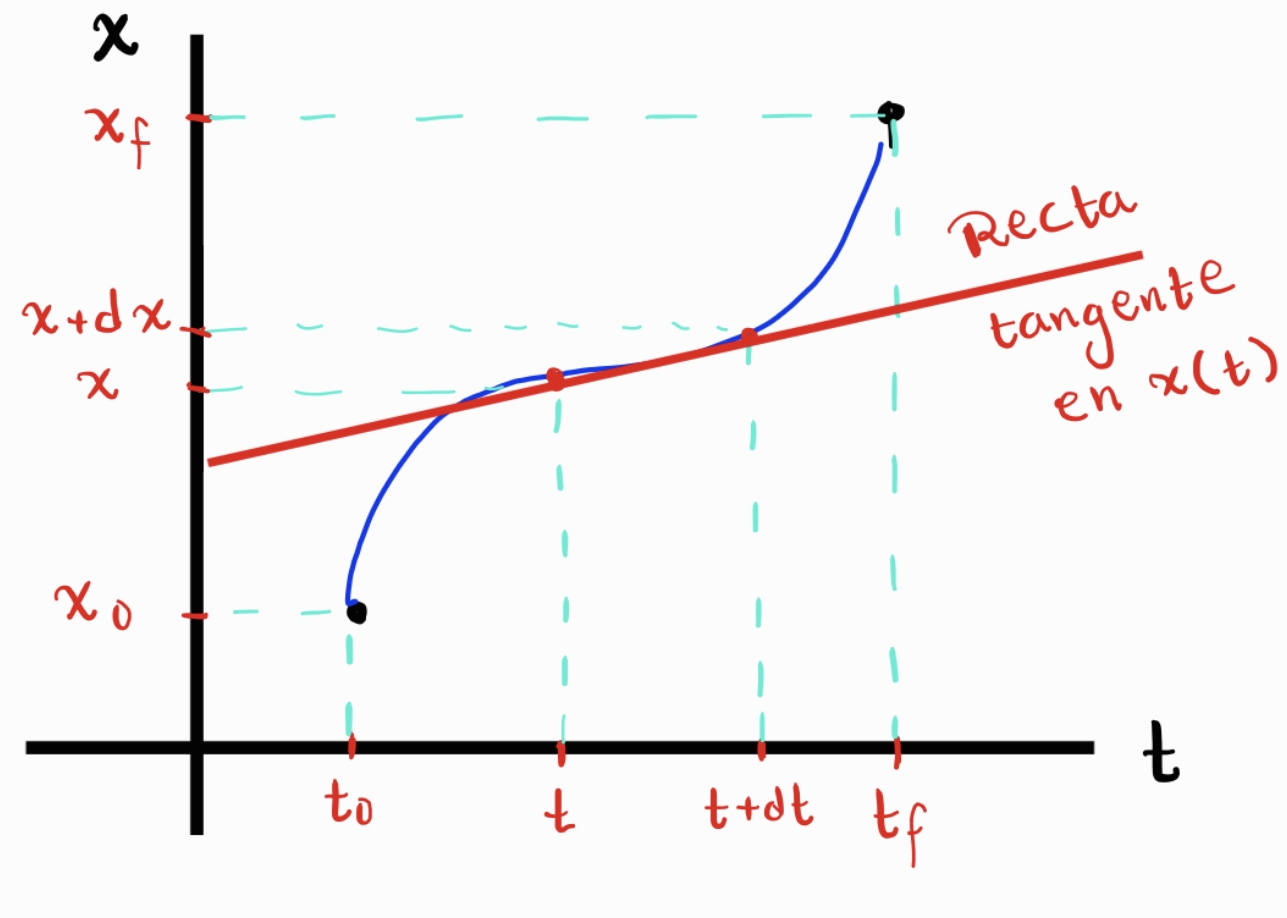
\includegraphics[width=0.5\linewidth]{figures/XvsT2.jpg}
    \end{figure}
    
    En general, para un objeto que se mueva en el espacio, la velocidad instantanea se define como la variación infinitesimal de la posición respecto de un incremento diferencial en el tiempo. Esto es,
    \begin{equation}
        v=\frac{dx}{dt}.
    \end{equation}
\end{frame}

\begin{frame}{Gráficas de $v$ vs $t$}

Una gráfica de velocidad contra tiempo muestra la evolución temporal de la velocidad instantanea de un sistema en el tiempo. El área bajo la curva de la gŕafica de velocidad contra tiempo en un intervalo de tiempo dado es el desplazamiento del cuerpo en ese intervalo.

\begin{figure}
    \centering
    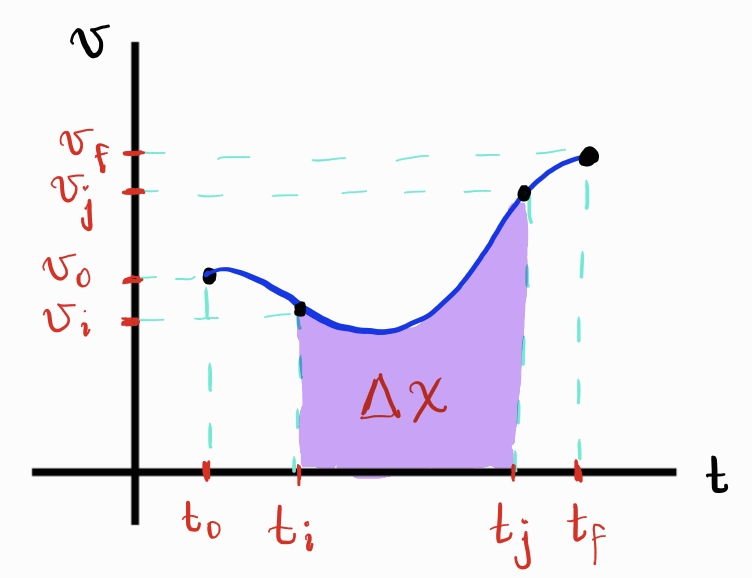
\includegraphics[width=0.4\linewidth]{figures/VvsT1.jpg}
\end{figure}

Por lo tanto, \begin{equation}
    x(t) = x_0 + \int_{t_0}^tv(t')\,dt'.
\end{equation}
    
\end{frame}

\begin{frame}{Posición de un sistema con velocidad constante}

Si un sistema se mueve con velocidad constante, esto es, $dv/dt=0$, su posición en función del tiempo está dada por la ecuación
    \begin{equation}
        x(t)=x_0+v(t-t_0).
    \end{equation}
    A este tipo de movimiento se le llama \textit{movimiento rectilineo uniforme}.
\end{frame}

\begin{frame}{Ejercicio 1}
    Considere un m\'ovil que se mueve en l\'inea recta sin aceleraci\'on. Se registra su posici\'on en diferentes instantes de tiempo tal que as\'i:
    \begin{itemize}
        \item Parte de $x = 2$ m y avanza 8 m hacia adelante en 4 s.
        \item Luego, retrocede 6 m en 3 s.
        \item Permanece en reposo en esa posici\'on durante 5 s.
        \item Finalmente, se mueve 10 m hacia adelante en 5 s.
    \end{itemize}
    
    Basado en la anterior descripci\'on,
    
    \begin{itemize}
        \item[a)] Grafique el movimiento descrito en una gr\'afica de posici\'on contra tiempo.
        \item[b)] Determine el desplazamiento en cada intervalo. 
        \item[c)] Calcule el desplazamiento total.
        \item[d)] Calcule la distancia total recorrida.
        \item[e)] Calcule la velocidad del móvil en cada tramo.
        \item[f)] Determine la ecuaci\'on de movimiento para cada tramo.
    \end{itemize}

\end{frame}

\begin{frame}{Ejercicio 2}
    Un m\'ovil inicia su movimiento hacia el este con una velocidad constante de $15 \,\text{m/s}$. 3.75 segundos despu\'es, un segundo m\'ovil parte hacia el oeste con velocidad constante de $25 \,\text{m/s}$. Si inicialmente los móviles distaban $20 \,\text{km}$, determine
    
    \begin{itemize}
        \item[a)] Cu\'anto tiempo les tomar\'a encontrarse.
        \item[b)] Cu\'al es la distancia recorrida por cada uno hasta el punto de encuentro.
        \item[c)] Cuánto tiempo le tomará al segundo alcanzar al primero si el primero inicialmente partiera hacia el oeste.
        \item[d)] Cuál es la distancia recorrida por cada uno en la situación del literal (c).
    \end{itemize}
\end{frame}

\begin{frame}{Concepto de aceleración}
    Considerar una partícula que al desplazarse, cambia su velocidad en incrementos iguales en tiempos iguales, es decir, el cambio de velocidad es directamente proporcional al cambio en el tiempo.

    \begin{figure}
        \centering
        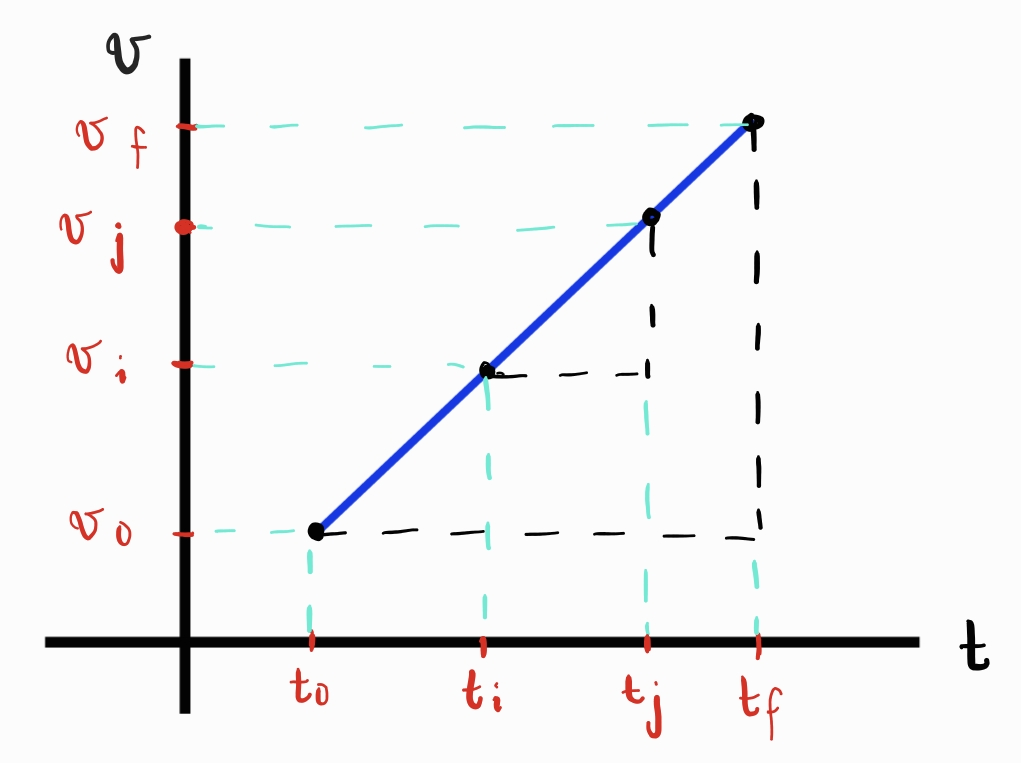
\includegraphics[width=0.4\linewidth]{figures/VvsT2.jpg}
    \end{figure}

    En esta situación, la \textbf{aceleración} se define como la variación de la velocidad respecto de la variación en el timpo dentro de los mismos intervalos, es decir, $$a=\frac{v_f-v_0}{t_f-t_0}=\frac{v_j-v_i}{t_j-t_i}=\frac{\Delta v}{\Delta t}.$$
    
\end{frame}

\begin{frame}{Aceleración instantanea}


    \begin{figure}
        \centering
        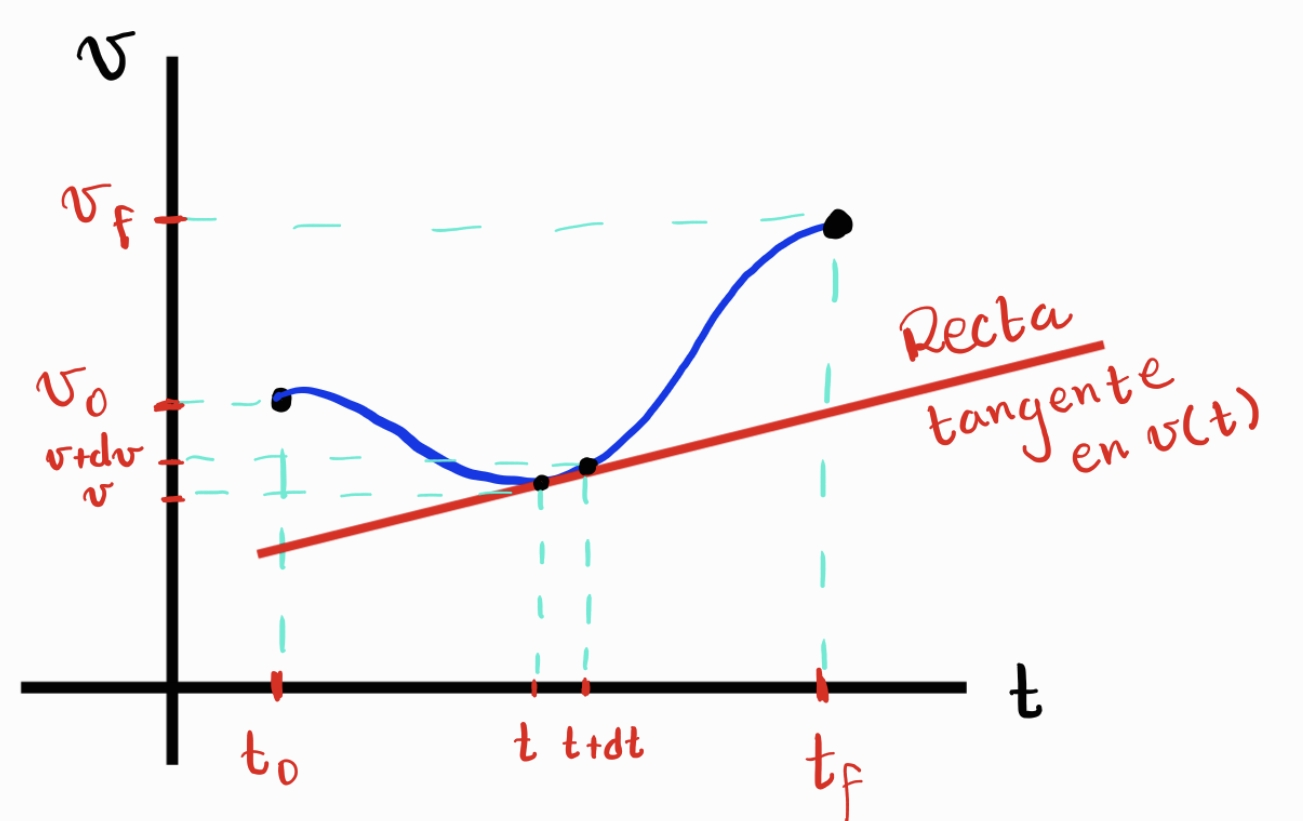
\includegraphics[width=0.5\linewidth]{figures/VvsT3.jpg}
    \end{figure}
    
    En general, para un objeto que se mueva en el espacio, la aceleración instantanea se define como la variación infinitesimal de la velocidad respecto de un incremento diferencial en el tiempo. Esto es,
    \begin{equation}
        a=\frac{dv}{dt}.
    \end{equation}
\end{frame}

\begin{frame}{Gráficas de $a$ vs $t$}

Una gráfica de aceleración contra tiempo muestra la evolución temporal de la aceleración instantanea de un sistema en el tiempo. El área bajo la curva de la gŕafica de aceleración contra tiempo en un intervalo de tiempo dado es el cambio en la velocidad del cuerpo en ese intervalo.

\begin{figure}
    \centering
    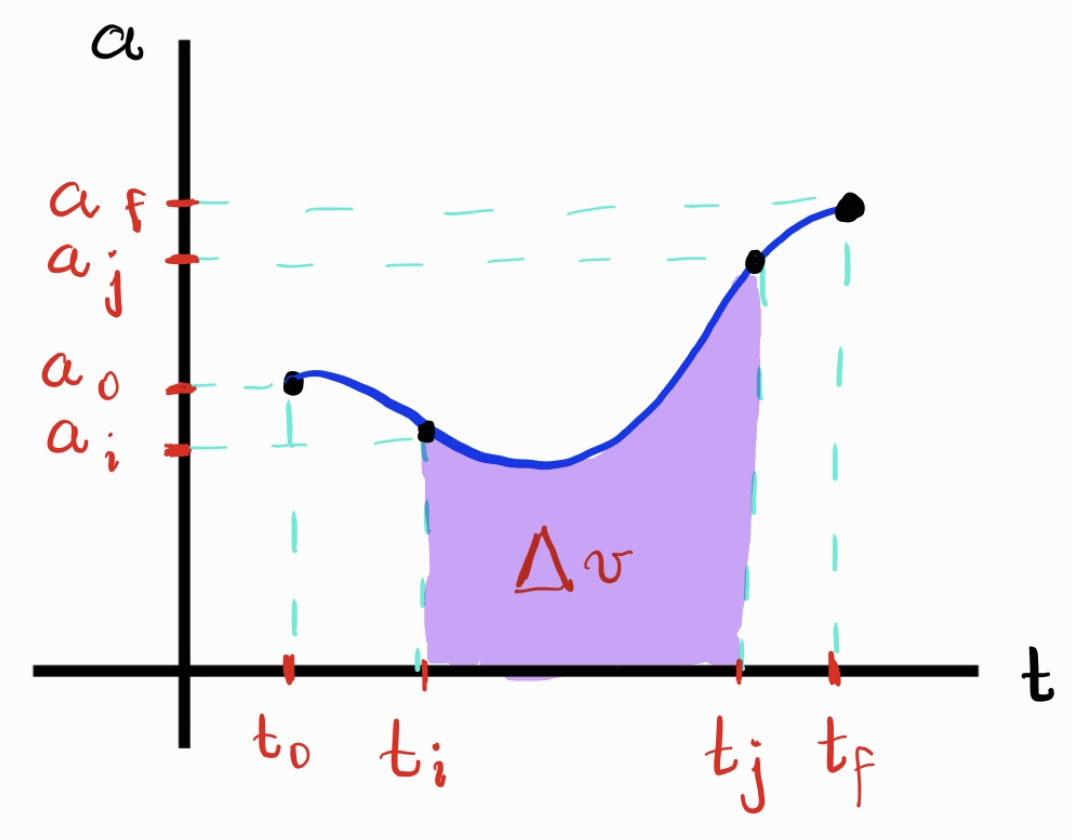
\includegraphics[width=0.4\linewidth]{figures/AvsT1.jpg}
\end{figure}

Por lo tanto, \begin{equation}
    v(t) = v_0 + \int_{t_0}^ta(t')\,dt'.
\end{equation}

\end{frame}

\begin{frame}{Posición de un sistema con aceleración constante}

Si un sistema se mueve con aceleración constante, esto es, $da/dt=0$, su posición en función del tiempo está dada por la ecuación
    \begin{equation}
        x(t)=x_0+v_0(t-t_0)+\frac{1}{2}a(t-t_0)^2.
    \end{equation}
    A este tipo de movimiento se le llama \textit{movimiento rectilineo uniformemente acelerado}.

    
    Nótese que si $a=0$, la ecuación de movimiento se transforma en la misma ecuación del movimiento rectilineo uniforme.
\end{frame}

\begin{frame}{Relación entre posición y velocidad de un sistema con aceleración constante}
    Si un sistema se mueve con aceleración constante, esto es, $da/dt=0$, su posición en función de la velocidad está dada por \begin{equation}
        [v(x)]^2=v_0^2+2a(x-x_0).
    \end{equation} 
\end{frame}

\begin{frame}{Ejercicio 1}
    Un objeto A es arrojado verticalmente hacia arriba con una velocidad de $6$ ft/s. Justo cuando llega al punto más alto, otro objeto B es arrojado verticalmente hacia arriba con una velocidad de $3.2$ ft/s.
	    
	    Determine
	    
	    \begin{itemize}
	    \item[a)] El tiempo para el cual ambos cuerpos se encuentran en su recorrido.
	    \item[b)] La posición en la que se encuentran.
	    \item[c)] Qué sucederá primero: ¿El cuerpo A llega al suelo o el cuerpo B llega el punto más alto?
	    \end{itemize}
	    
\end{frame}

\begin{frame}{Idealización}
    En física, una idealización es una simplificación intencionada de un fenómeno o sistema real para hacerlo más manejable o fácil de analizar, asumiendo que ciertos detalles poco relevantes son irreales o pueden ignorarse. Por ejemplo: \begin{itemize}
        \item Una superficie muy lisa carece de rozamiento.
        \item Un objeto que cae en las profundidades del mar no se ve afectado por las corrientes marítimas
        \item Una superficie plana es perfectamente plana.
        \item Un agujero negro es perfectamente esférico (radio de Schwarzschild).
    \end{itemize}

    $$\vdots$$
\end{frame}

\begin{frame}
    \begin{figure}
        \centering
        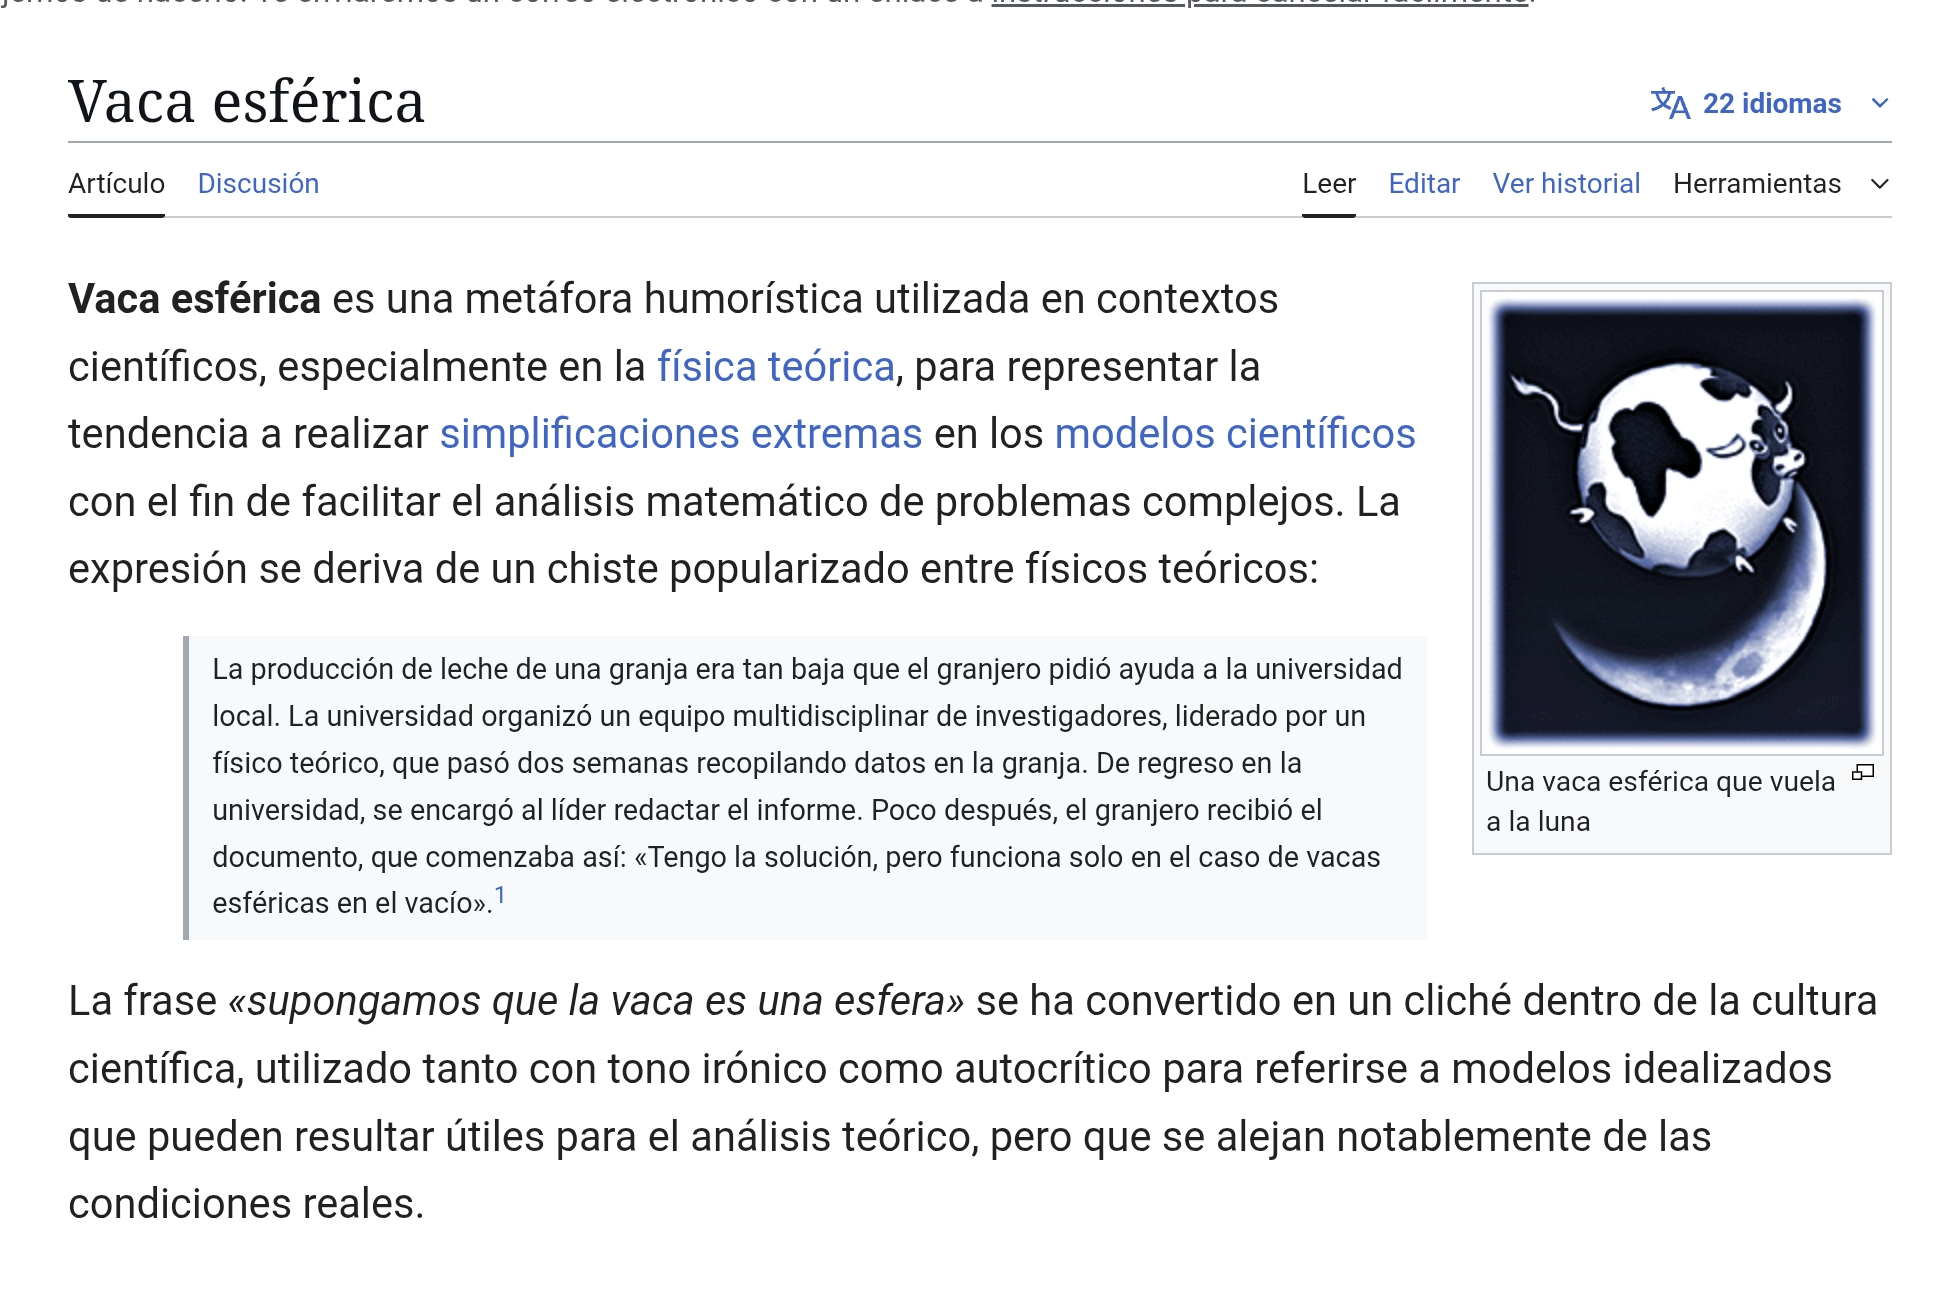
\includegraphics[width=\linewidth]{figures/vaca-esferica.jpg}
    \end{figure}
\end{frame}

\begin{frame}
    \begin{figure}
        \centering
        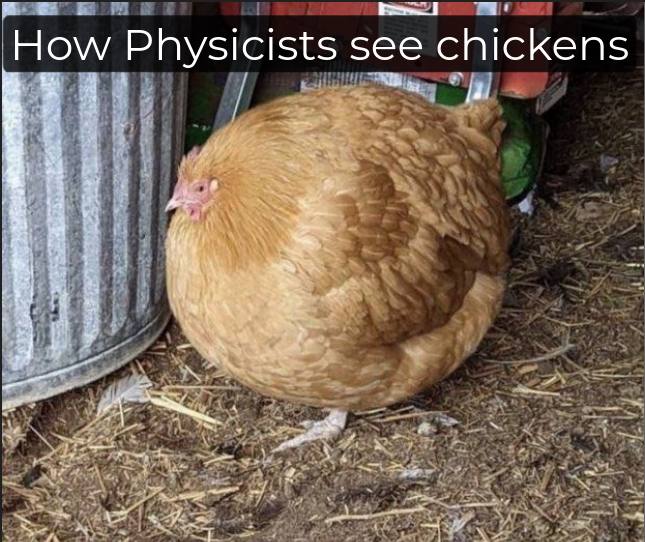
\includegraphics[width=0.8\linewidth]{figures/spherical-chiken.png}
    \end{figure}
\end{frame}

\begin{frame}{Idealizaciones (hasta nuevo aviso)}

A continuación, se detallan una serie de idealizaciones que usaremos (hasta nuevo aviso) en el curso.

\begin{enumerate}
    \item Los objetos que se mueven no tienen dimensión.
    \item El aire no existe.
    \item Las superficies lisas son perfectamente lisas.
    \item La aceleración gravitacional es la misma en todos los lugares del planeta tierra.
\end{enumerate}

    
\end{frame}

\begin{frame}{Caida libre}
    Diálogos sobre dos nuevas ciencias (1638) es la última obra de Galileo Galilei, donde resume décadas de investigaciones. En ella, presenta dos pilares clave: la resistencia de los materiales y el movimiento de los cuerpos.

Su impacto en la física fue enorme, ya que:

\begin{itemize}
    \item Introdujo una descripción matemática del movimiento uniformemente acelerado.
    \item Sentó las bases de la cinemática moderna.
    \item Fue precursor del método científico experimental.

    \item Influenció directamente a Newton en la formulación de sus leyes.

    \item La obra marcó el tránsito de la física aristotélica a la física moderna.
\end{itemize}

\end{frame}

\begin{frame}

"$[\dots]$ porque así, como la uniformidad 
del movimiento se define y se concibe por medio de la 
uniformidad de los tiempos y de los espacios (pues al movimiento 
le llamamos uniforme, cuando espacios iguales son recorridos 
en tiempos iguales), así también, por medio de la 
igualdad, de los intervalos del tiempo, podemos concebir los 
incrementos de la velocidad simplemente agregados; entendiendo 
que ese movimiento es acelerado uniformemente y del 
mismo modo continuamente, siempre que en cualesquiera 
tiempos iguales se le vayan sobreañadiendo aditamentos iguales 
de velocidad. De modo que si, tomado un número cualquiera 
de intervalos iguales de tiempo, a contar desde el primer 
instante en que el móvil abandona el reposo y comienza el descenso, 
la velocidad, adquirida durante el primero más el segundo 
intervalo de tiempo, es doble de aquella que el móvil adquirió 
durante el primer intervalo solo; la velocidad que adquiere 
durante tres intervalos de tiempo, es triple; y la que adquiere 
en cuatro, cuádruple de la velocidad del primer tiempo. 
    
\end{frame}

\begin{frame}
    De 
modo que (para más clara comprensión), si el móvil continua 
a su movimiento uniformemente con la velocidad adquirida 
en el primer intervalo de tiempo, este movimiento sería dos 
veces más tardo que aquel que hubiera alcanzado con la velocidad 
adquirida en dos intervalos de tiempo. Y así, no parece 
repugnar a la recta razón el admitir que el incremento de la velocidad 
se efectúa según la extensión del tiempo; de donde, la
definición del movimiento que vamos a tratar, puede ser la siguiente: 

\bigskip

\begin{itemize}
    \item[] \textit{Llamo movimiento igualmente o uniformemente acelerado 
aquel que, a partir del reposo, va adquiriendo incrementos 
iguales de velocidad durante intervalos iguales de tiempo.}"
\end{itemize}

\bigskip
\bigskip

\raggedleft{{\textit{Diálogos sobre dos nuevas ciencias}, \textbf{Galileo Galilei (1638)}}}

\end{frame}

\begin{frame}{Conclusión clave}
    \LARGE \textbf{Cuando un objeto cae en el seno de un campo gravitacional uniforme, describe un movimiento uniformemente acelerado.}
\end{frame}

\begin{frame}{Ecuaciones de movimiento}
    La ecuación de movimiento para un objeto que asciende o desciende en caida libre está dada por \begin{equation}
        y(t)=y_0+v_0(t-t_0)-\frac{1}{2}g(t-t_0)^2,
    \end{equation} donde $g$ es la aceleración gravitacional y la referencia $y=0$ está en el punto más bajo del espacio (normalmente, el suelo).
    
    \vspace{1em}
    
    En el planeta Tierra, $$g=\num{9.81}\,\unit{m}/\unit{s}^2.$$
\end{frame}

\begin{frame}{Ejercicio 1}
    Un tubo que gotea, libera gotas de agua cada 3 s. Determine la distancia que separará a dos gotas consecutivas, pasados 7.2 s desde que cae la primera gota.
\end{frame}

\begin{frame}{Ejercicio 2}
    Un hombre se mueve en  motocicleta con rapidez 
constante de 54 $\unit{km}/\unit{h}$ hacia un 
edificio de 40 m de altura. Una 
persona en la azotea del edificio 
lanza verticalmente una pelota con 
la intención de que caiga en una 
canasta situada a 1 m del suelo en 
la motocicleta. La persona en la 
azotea lanza la pelota desde una 
altura de 42 m y la motocicleta está 
a 30 m del edificio. Determine la velocidad con la que debe lanzarse la pelota para que esta caiga en 
la canasta cuando la motocicleta está en la base del edificio.

\begin{figure}
    \centering
    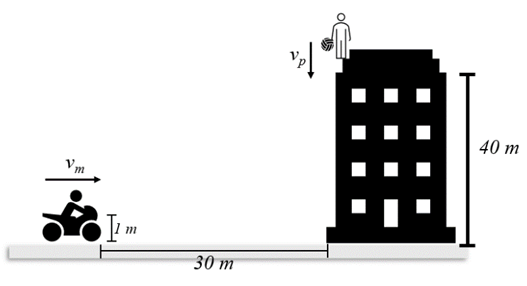
\includegraphics[width=0.7\linewidth]{figures/moto-edificio.png}
\end{figure}

\end{frame}

\begin{frame}{Movimiento parabólico}
\begin{figure}
    \centering
    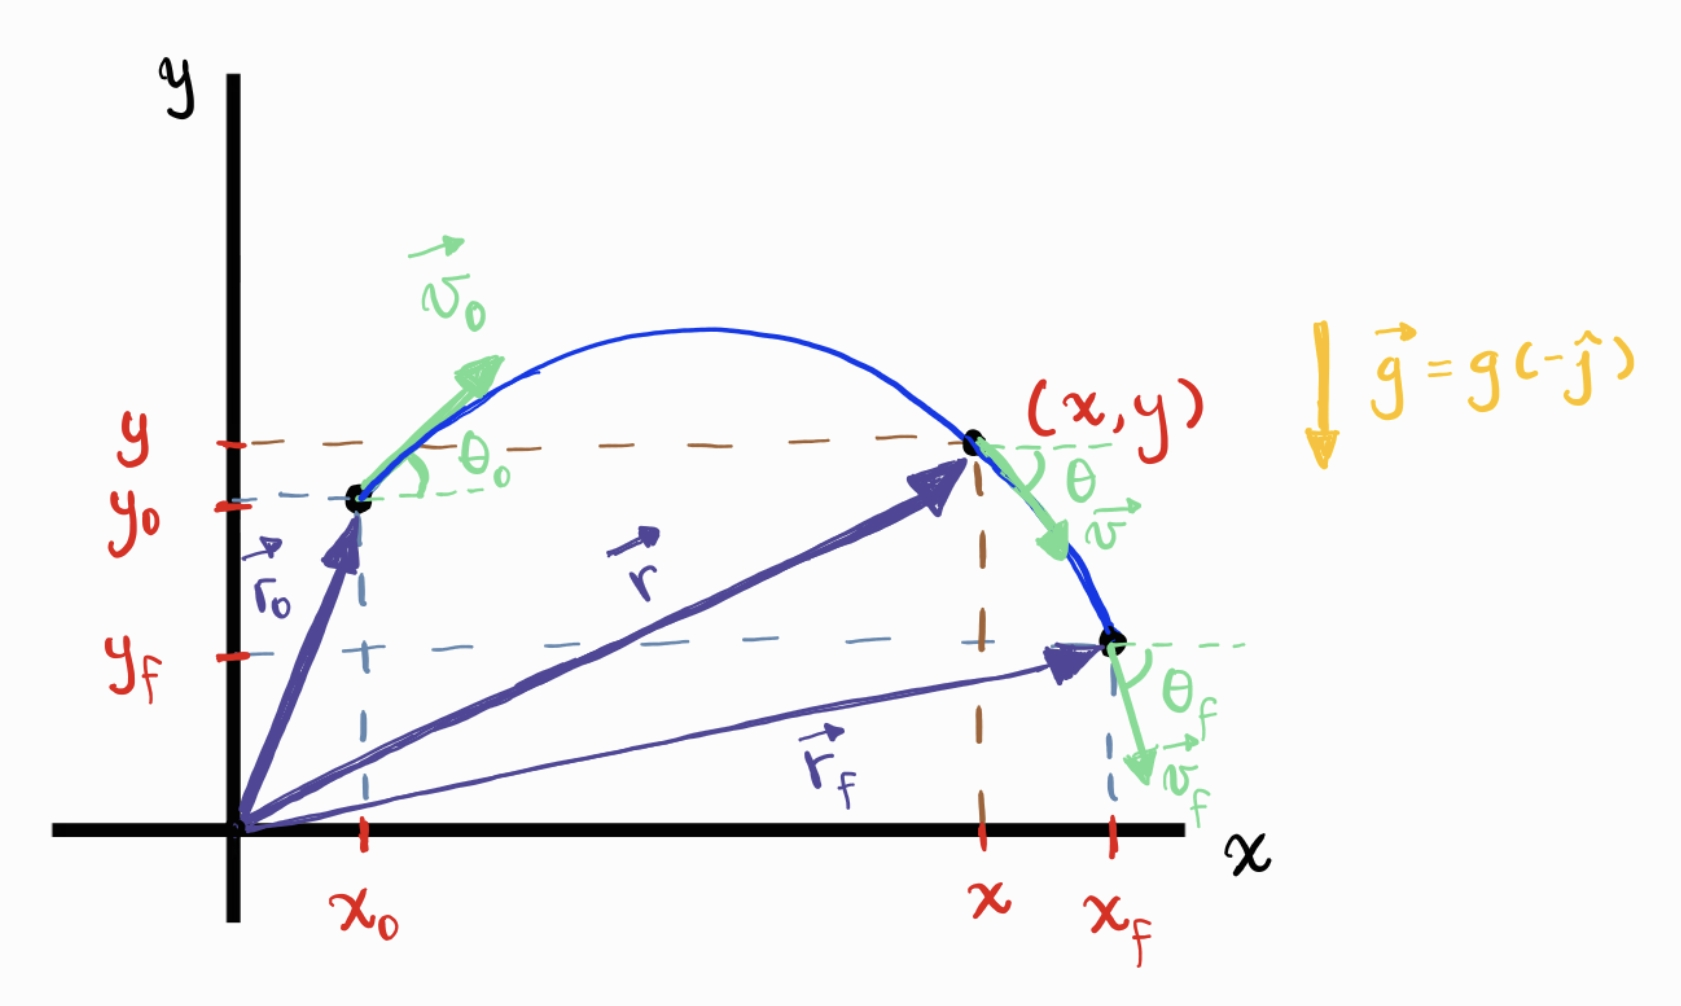
\includegraphics[width=0.7\linewidth]{figures/Parabolico.jpg}
\end{figure}
    El movimiento parabólico es un tipo de movimiento bidimensional en el que la ubicación del objeto que describe tal movimiento está dada por un vector de posición dependiente del tiempo, $$\vec{r}(t)=x(t)\hat{\imath}+y(t)\hat{\jmath}.$$
\end{frame}

    \begin{frame}{Posición en el movimiento parabólico}
    
    La evolución temporal del vector de posición está dada tal que así: \begin{itemize}
        \item La componente horizontal evoluciona de acuerdo con un MRU, \begin{equation}
            x(t)=x_0+v_x(t-t_0).
        \end{equation}
        \item La componente vertical evoluciona temporalmente de acuerdo con un MRUA influenciado por la aceleración gravitacional, \begin{equation}
            y(t)=y_0+v_{0y}(t-t_0)-\frac{1}{2}g(t-t_0)^2.
        \end{equation}
    \end{itemize}
    El vector de velocidad evoluciona como

    \begin{align}
        \nonumber v(t)&=\frac{d\vec{r}}{dt}=\frac{dx}{dt}\hat{\imath}+\frac{dy}{dt}\hat{\imath}=v_x\hat{\imath}+v_y\hat{\jmath}\\
        &=v_x\hat{\imath}+(v_{0y}-g(t-t_0))\hat{\jmath}.
    \end{align}
\end{frame}

\begin{frame}{Ejercicio 1}
    Un proyectil arrojado con un ángulo de $\pi/4\,\unit{rad}$ sobre la horizontal, a una velocidad de 9 $\unit{m}/\unit{s}$. Determine:
	
	\begin{itemize}
	    \item[a)] La altura máxima que alcanza.
	    \item[b)] El tiempo de vuelo.
	    \item[c)] El desplazamiento horizontal máximo.
	\end{itemize}
\end{frame}

\begin{frame}{Ejercicio 2}
    Un hombre está de pie en la azotea de un edificio de 
$15.0 \,\text{m}$ de altura y lanza una piedra con una velocidad de 
$30.0 \,\text{m/s}$ a un ángulo de $33.0^\circ$ sobre la horizontal. 
Puede ignorar la resistencia del aire. Calcule 
\begin{itemize}
    \item[a)] la altura máxima que alcanza la piedra sobre la azotea;
    \item[b)] la magnitud de la velocidad de la piedra justo antes de golpear el suelo; y
    \item[c)] la distancia horizontal desde la base del edificio hasta el punto donde la piedra golpea el suelo.
    \item[d)] Dibuje las gráficas $x$--$t$, $y$--$t$, $v_x$--$t$ y $v_y$--$t$ para el movimiento.
\end{itemize}
\end{frame}

\begin{frame}{Ejercicio 3}
 Un pasajero en un 
tren que se mueve a 80 
$\unit{km}/\unit{h}$ lanza verticalmente 
hacia arriba una pelota 
desde una ventana 
situada a 1.5 m de altura 
respecto del suelo con 
una velocidad de 6 $\unit{m}/\unit{s}$. 
La pelota debe caer en 
una caja de 1.0 m de altura y 50 cm de ancho, situada a 25 m horizontales del punto de 
lanzamiento. ¿Cae la pelota dentro de la caja?

\begin{figure}
    \centering
    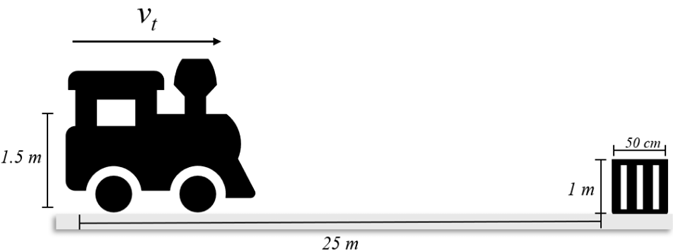
\includegraphics[width=0.8\linewidth]{figures/tren-caja.png}
\end{figure}
   
\end{frame}

\begin{frame}{Movimiento circular}

    \begin{figure}
        \centering
        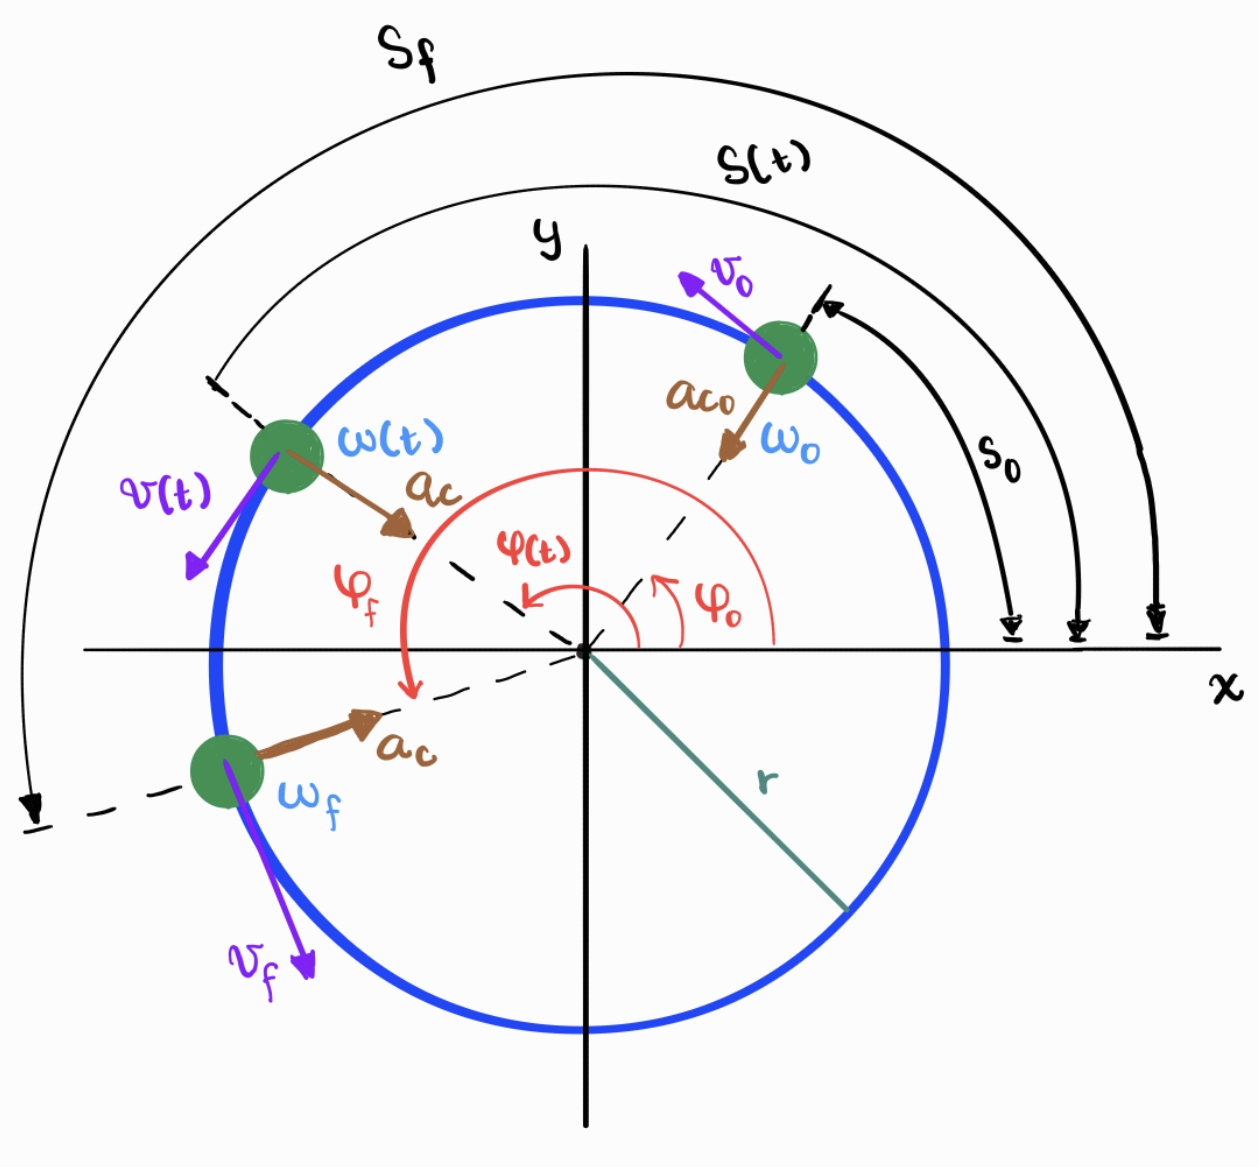
\includegraphics[width=0.5\linewidth]{figures/mcua.jpg}
    \end{figure}

    \footnotesize
\vspace{-1em}
    Un sistema que se mueve describiendo un movimiento circular puede parametrizarse utilizando las siguientes variables.
    
    
    \begin{columns}
    \footnotesize
        \column{0.48\textwidth}
        \textbf{Lineales}
        \begin{itemize}
            \item $s\,[\unit{m}]$: Posición radial
            \item $v\,[\unit{m}/\unit{s}]$: Velocidad tangencial
            \item $a\,[\unit{m}/\unit{s}^2]$: Aceleración tangencial
        \end{itemize}
        \column{0.48\textwidth}
        \textbf{Angulares}
        \begin{itemize}
            \item $\varphi\,[\unit{rad}]$: Posición angular
            \item $\omega\,[\unit{rad}/\unit{s}]$: Velocidad angular
            \item $\alpha\,[\unit{rad}/\unit{s}^2]$: Aceleración angular
        \end{itemize}
    \end{columns}
    
\end{frame}

\begin{frame}{Ecuaciones de movimiento}
    Las ecuaciones de movimiento son equivalentes a las estudiadas:
    \vspace{1em}
    \begin{columns}
        \column{0.48\textwidth}
        \textbf{Lineales}
        \begin{itemize}
            \item $v=\cfrac{ds}{dt}$
            \item $a=\cfrac{dv}{dt}=\cfrac{d^2s}{dt^2}$
        \end{itemize}
        \column{0.48\textwidth}
        \textbf{Angulares}
         \begin{itemize}
            \item $\omega=\cfrac{d\varphi}{dt}$
            \item $\alpha=\cfrac{d\omega}{dt}=\cfrac{d^2\varphi}{dt^2}$
        \end{itemize}
    \end{columns}
    \vspace{1em}
    Si la aceleración del sistema es constante, la solución a estas ecuaciones diferenciales resulta en la forma ya conocida.

    \vspace{1em}
    \begin{columns}
    
        \column{0.48\textwidth}
        \textbf{Lineales}
        \small
        \begin{itemize}
            \item $s=s_0+v_0(t-t_0)+\cfrac{1}{2}a(t-t_0)^2$
            \item $v=v_0+a(t-t_0)$
            \item $v^2=v_0^2+2a(s-s_0)$
        \end{itemize}
        \column{0.48\textwidth}
        \textbf{Angulares}
        \small
         \begin{itemize}
            \item $\varphi=\varphi_0+\omega_0(t-t_0)+\cfrac{1}{2}\alpha(t-t_0)^2$
            \item $\omega=\omega_0+\alpha(t-t_0)$
            \item $\omega^2=\omega_0^2+2\alpha(\varphi-\varphi_0)$
        \end{itemize}
    \end{columns}
\end{frame}

\begin{frame}{Aceleración centrípeta}
    En este movimiento se presenta un nuevo tipo de aceleración lineal asociado a una fuerza ficticia:
    \begin{center}
        $a_c\,[\unit{m}/\unit{s}^2]$: Aceleración centrípeta.
    \end{center}
    Este tipo de aceleración verifica las siguiente ecuación:

    \begin{equation}
        a_c=\frac{v^2}{r}=\omega^2r.
    \end{equation}
    De aquí, se deduce que \begin{align}
        v&=\omega r,\\
        a&=\alpha r.
    \end{align}
    
\end{frame}

\begin{frame}{Aceleración total}
    La aceleración total del sistema está dada por
    \begin{equation}
        a_{\text{total}}=\sqrt{a^2+a_c^2}.
    \end{equation}
\end{frame}

\begin{frame}{Periodo y frecuencia}
    El periodo se define como el tiempo que le toma a un objeto desarrollar cierta cantidad de revoluciones, estos es, \begin{equation}
        T=\frac{\text{Tiempo}}{\text{Número de revoluciones}}.
    \end{equation} La frecuencia es el recíproco del periodo: el número de revoluciones que ejecuta un objeto en cierta cantidad de tiempo, es decir, \begin{equation}
        f=\frac{\text{Número de revoluciones}}{\text{Tiempo}}.
    \end{equation} Por lo tanto, \begin{equation}
        f=\frac{1}{T}
    \end{equation}
\end{frame}

\begin{frame}{Ejercicio 1}
    El periodo de traslación de la tierra es de 365.25 días. La distancia de la tierra al sol es de $148.03\times 10^6$ km. Calcular
	    \begin{itemize}
	        \item[a)] La frecuencia angular de la tierra en rad/s
	        \item[b)] La velocidad de traslación de la tierra en km/s
	        \item[c)] El aceleración centrípeta de la tierra en m/s$^2$
	\end{itemize}
\end{frame}

\begin{frame}{Ejercicio 2}
    Dos móviles describen una trayectoria circular y salen del mismo punto, en sentidos opuestos con velocidades de $\pi/6$ y $\pi/3$ rad/s. Si el radio de la circunferencia es de 2 m, calcular
\begin{itemize}
    \item[a)] El tiempo que tardan en encontrarse.
    \item[b)] El ángulo barrido por cada uno.
    \item[c)] La distancia que cada uno recorre.
    \end{itemize}
\end{frame}

\begin{frame}{Quiz 1: Consistencia}
    Investigar en qué consiste el \textit{movimiento relativo} desde el texto guía de Sears and Zemansky (o Serway):

    \begin{enumerate}
        \item (0.5) Definición.
        \item (0.5) Dos ejemplos cualitativos de movimiento relativo en la vida cotidiana.
        \item (1.0) Dos ejemplos cuantitativos de movimiento relativo con procedimiento analítico (pueden ser obtenidos del texto guía).
        \item (3.0) Resolver el problema que se presenta en la diapositiva siguiente.
    \end{enumerate}
\end{frame}

\begin{frame}{Quiz 1: Problema propuesto}
    Antonio en su Corvette acelera de acuerdo a $(3.00\hat{\imath}-2.00\hat{\jmath})$ m/s$^2$ mientras Jill en su Jaguar acelera a $(1.00\hat{\imath}+3.00\hat{\jmath})$ m/s$^2$. Ambos parten del reposo en el origen de un sistema coordenado $xy$. Después de $5.00$ s,
	\begin{itemize}
	    \item[a)] ¿Cuál es la rapidez de Antonio respecto de Jill?
	    \item[b)] ¿Qué distancia los separa?
	    \item[c)] ¿Cuál es la aceleración de Antonio en relación con Jill?
	\end{itemize}
\end{frame}

\begin{frame}{Quiz 1: Rúbrica de evaluación}
\tiny
    \begin{table}[H]
\centering
\renewcommand{\arraystretch}{1.4}
\begin{tabular}{|M{2cm}|c|m{7cm}|}
\hline
\textbf{Criterio} & \textbf{Puntaje} & \textbf{Descripción de desempeño} \\ \hline
Definición de movimiento relativo & 0.5 & Presenta una definición clara, precisa y acorde al texto guía. Se evalúa la corrección conceptual. \\ \hline
Dos ejemplos cualitativos & 0.5 & Muestra dos ejemplos de la vida cotidiana que reflejen adecuadamente el concepto de movimiento relativo. Deben ser pertinentes y explicados con claridad. \\ \hline
Dos ejemplos cuantitativos con procedimiento & 1.0 & Incluye dos ejercicios analíticos completos. Deben estar resueltos paso a paso, con justificación matemática y resultado correcto. \\ \hline
Resolución del problema asignado & 3.0 & Resuelve el problema planteado. Se evalúa: \begin{itemize}
    \item Comprensión del enunciado
    \item Aplicación correcta de fórmulas
    \item Desarrollo paso a paso
    \item Claridad en la presentación del resultado
\end{itemize} \\ \hline
\textbf{Total} & \textbf{5.0} & \\ \hline
\end{tabular}
\end{table}

\begin{center}
    \textbf{\large Este quiz se monta a la plataforma de Ude@ a más tardar el sábado 06 de septiembre}.
\end{center}

\end{frame}

\begin{frame}{Clase taller}
    En un bar local, un cliente desliza sobre la barra un tarro de cerveza vacío para que lo vuelvan a llenar. El cantinero está momentáneamente distraído y no ve el tarro, que se desliza de la barra y golpea el suelo a 1.40 m de la base de la barra.
        Si la altura de la barra es de 0.860 m,
        
        \begin{itemize}
            \item [a)] ¿Con qué velocidad el tarro dejó la barra?
            \item [b)] ¿Cuál fue la dirección de la velocidad del tarro justo antes de golpear el suelo? 
        \end{itemize}
\end{frame}

\begin{frame}{Clase taller}
    Un cohete de fuegos artificiales explota a una altura $h$, el máximo de su trayectoria vertical. Lanza fragmentos ardientes en
todas direcciones, pero todas con la misma rapidez $v_0$. Gránulos
de metal solidificado caen al suelo sin resistencia del aire. Encuentre el ángulo más pequeño que forma con la horizontal
la velocidad final de un fragmento.
\end{frame}

\begin{frame}{Clase taller}
    Un electrón ingresa a un condensador por su punto medio, con una velocidad de $(2.10\times10^{7}$ $m/s)\hat{i}$, en el que experimenta una aceleración de $(3.52\times10^{15}$ $m/s^2)\hat{j}$. El condensador posee una longitud de $6.0$ $cm$ y la separación entre las placas es de $2.0$ $cm$. A $12.0$ $cm$ del extremo derecho del condensador, hay una pantalla de detección. Suponiendo que el electrón no se ve afectado por la fuerza de atracción gravitacional, determine:
	    
	    \begin{itemize}
	        \item[a)] La velocidad con la que sale del condensador.
	        \item[b)] La distancia a la que es detectado en la pantalla, respecto a la línea horizontal que divide el condensador en dos mitades iguales.
	    \end{itemize}
        \begin{figure}[H]
  \centering
    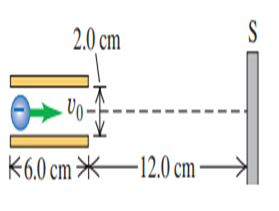
\includegraphics[width=0.3\textwidth]{figures/E.png}
\end{figure}
\end{frame}

\begin{frame}
\begin{center}
    \Huge \textbf{Capítulo 4}
    
    \LARGE Dinámica

    \textit{Leyes del movimiento de Newton}
\end{center}
    
\end{frame}

\begin{frame}{Dinámica}
    ¿Qué ocasiona que los cuerpos se muevan como lo hacen?

    Tres formalismos
    \begin{center}
    
        \textbf{Newton}
        \begin{equation*}
            \boxed{\vec{F}=m\vec{a}}
        \end{equation*}

        \textbf{D'Alembert}
        \begin{equation*}
        \vec{R}_i\cdot\delta\vec{r}_i=0
        \end{equation*}
        
        \textbf{Hamilton y Lagrange}
        \begin{align*}
            &\frac{\partial\mathcal{L}}{\partial q}-\frac{d}{dt}\left(\frac{\partial\mathcal{L}}{\partial\dot{q}}\right)=0\\
            &\mathcal{H}=p\dot{q}-\mathcal{L}
        \end{align*}
    \end{center}
        
\end{frame}

\begin{frame}{Sistema y entorno}
    Un \emph{sistema} puede estar conformado por uno o más objetos. Todo lo que no está incluido en el sistema es parte del \textbf{entorno}.
\end{frame}

\begin{frame}{Concepto de fuerza}
    Fuerza $\mathbf{F}$: La fuerza cuantifica la cantidad de interacción entre dos objetos. Como la fuerza tiene una determinada magnitud y se ejerce en una dirección, entonces es un vector

Ejemplos:
\begin{itemize}
\item Fuerza repulsiva entre un protón y otro protón.
\item La fuerza gravitacional atractiva que la tierra ejerce sobre usted.
\item La fuerza que un resorte comprimido ejerce sobre su mano.
\item La fuerza en una nave espacial de los gases expandiéndose en la
  maquinaria del cohete.
\end{itemize}
\end{frame}

\begin{frame}{Tipos de fuerza}

\begin{columns}
    \column{0.45\textwidth}
    \textbf{Fuerza normal ($\vec{n}$)}: Cuando un objeto descansa o se empuja sobre una superficie, esta ejerce un empujón sobre el objeto que es perpendicular a la superficie.
    \begin{figure}
        \centering
        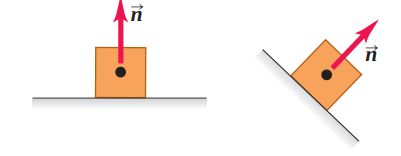
\includegraphics[width=0.8\linewidth]{figures/normal.png}
    \end{figure}
    
    \column{0.45\textwidth}
    \textbf{Fuerza de fricción ($\vec{f}$)}: Además de la fuerza normal, una superficie puede ejercer una fuerza de fricción sobre un objeto que es paralela a la superficie.
    \begin{figure}
        \centering
        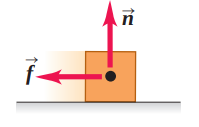
\includegraphics[width=0.5\linewidth]{figures/friccion.png}
    \end{figure}
\end{columns}
    
\end{frame}

\begin{frame}
    \begin{columns}
    \column{0.45\textwidth}
    \textbf{Fuerza de tensión ($\vec{T}$)}: La fuerza de un tirón ejercida sobre un objeto por una cuerda, un cordón, etcétera.
    \begin{figure}
        \centering
        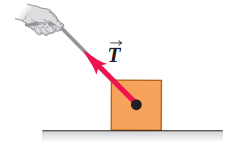
\includegraphics[width=0.8\linewidth]{figures/tension.png}
    \end{figure}
    
    \column{0.45\textwidth}
    \textbf{Peso ($\vec{w}$)}: El tirón de la gravedad sobre un objeto es una fuerza de largo alcance (una fuerza que actúa a la distancia).
    \begin{figure}
        \centering
        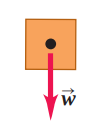
\includegraphics[width=0.4\linewidth]{figures/peso.png}
    \end{figure}
\end{columns}
\end{frame}

\begin{frame}
    \begin{center}
        \Huge ¿Preguntas?
    \end{center}
\end{frame}

\begin{frame}{Medición de la fuerza}
    Para describir una fuerza vectorial, debemos indicar la dirección en la cual actúa, así como su magnitud, es decir, la cantidad que describe “cuánto” o “qué tanto” la fuerza empuja o tira. La unidad de magnitud de fuerza en el SI es el newton, que se abrevia N. Usualmente se utiliza el \textit{dinamómetro} para medir fuerzas. \textbf{Ejemplos:}

    \begin{figure}
        \centering
        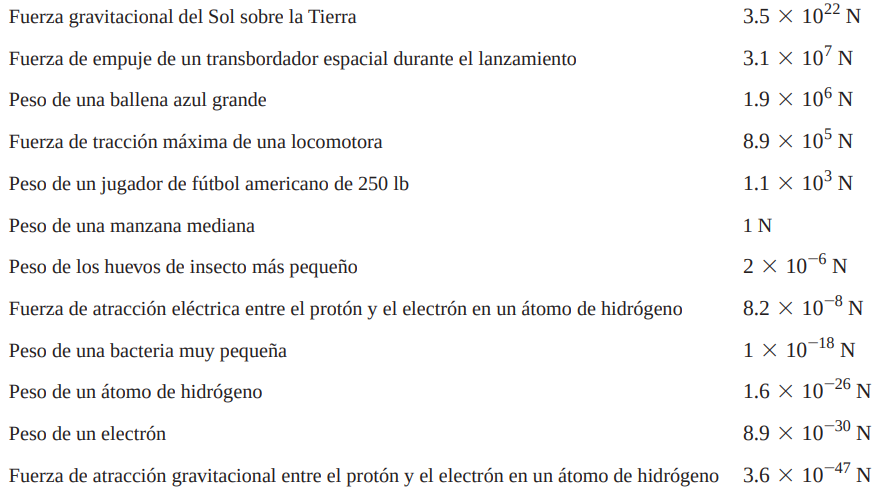
\includegraphics[width=0.8\linewidth]{figures/image.png}
    \end{figure}
\end{frame}

\begin{frame}{Superposición de fuerzas}
    Puesto que las fuerzas son cantidades vectoriales (vectores libres), pueden ser sumadas tal que en un sistema, la fuerza total o resultante resulta ser \begin{equation}
        \vec{F}_{\text{Total}}=\sum_{i=1}^N\vec{F}_i=\vec{F}_1+\vec{F}_2+\vec{F}_3+\dots+\vec{F}_{N-1}+\vec{F}_N.
    \end{equation}

    \begin{figure}
        \centering
        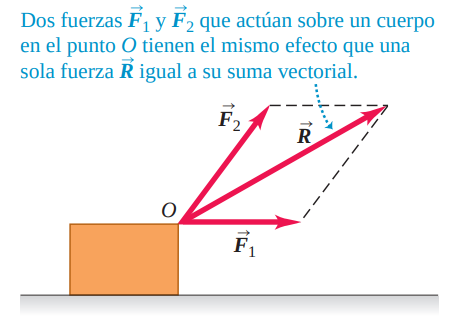
\includegraphics[width=0.4\linewidth]{figures/superposicion.png}
    \end{figure}
    En la figura, $\vec{R}$ está dada por 
    \begin{equation}
    \vec{R}=(F_{1x}+F_{2x})\hat{\imath}+(F_{1y}+F_{2y})\hat{\jmath}.
\end{equation}
\end{frame}

\begin{frame}{Sistemas inerciales}
Considere ahora dos sistemas de referencia con $S:(x,y,z,t)$ en reposo
y $S':(x',y',z',t')$ moviéndose a velocidad constante
$\mathbf{V}$.
\vspace{1em}

    \pause Sea $\mathbf{r}$ el vector de posición de un cuerpo relativo al
primer sistema de referencia, y $\mathbf{r}'$ su vector de posición
relativo al segundo.
Asumiendo que los sistemas de referencia coinciden en el tiempo
$t=t'=0$, entonces
\begin{align}
  \mathbf{r}(t)=\mathbf{r}'(t)+\mathbf{R}(t)\,,
\end{align}

\pause donde el sistema de coordenadas primado se mueve con velocidad
$\mathbf{V}$ a largo de $\mathbf{R}$:
\begin{align}
  \mathbf{R}(t)=\mathbf{V}\, t\,,
\end{align}
\end{frame}

\begin{frame}
    Al derivar,
    \begin{align}
  \mathbf{v}'(t)=\mathbf{v}(t)-\mathbf{V}\,.
\end{align}
Pero para la aceleración:
\begin{align}
  \mathbf{a}'=\mathbf{a}\,,
\end{align} de modo que \textbf{si la velocidad relativa entre los sistemas es constante,
la aceleración de un objeto vista desde los dos sistemas de referencia
es la misma}.

\vspace{1em}

\begin{center}
    \Large Hemos definido qué es un sistema inercial.
\end{center}

\pause \textit{(Un sistema de coordenadas
inercial es un sistema de coordenadas que se mueve a velocidad
constante)}
\end{frame}

\begin{frame}
    \begin{center}
        \Huge ¿Preguntas?
    \end{center}
\end{frame}

\begin{frame}
    \begin{center}
        {\Huge \textbf{LEYES DE NEWTON}}
        
        (así, \textit{en mayúscula})
    \end{center}
\end{frame}

\begin{frame}{Primera ley de Newton}
    \textbf{Ley de la inercia}: Los cuerpos aislados se mueven
uniformemente con respecto a sistemas inerciales.

\vspace{1em}

Un cuerpo sobre el que no actúan fuerzas se llama \emph{cuerpo libre}.

\vspace{1em}

Dicho de otra forma:
\begin{center}
    \textit{Un cuerpo sobre el que no actúa una fuerza neta se mueve con velocidad constante (que puede ser cero) y aceleración cero.}
\end{center}
\vspace{1em}

Esto es, \begin{equation*}
    \sum_i\vec{F}_i=\vec{0}\Rightarrow\vec{a}=\frac{d\vec{v}}{dt}=\vec{0}
\end{equation*}

La tendencia de un cuerpo a seguir moviéndose una vez iniciado su movimiento es resultado de una propiedad llamada \textbf{inercia}.

\end{frame}

\begin{frame}{Ejemplos}
    \section*{Ejemplos de la Ley de Inercia de Newton}

\textbf{Objetos en Reposo}
\begin{itemize}
    \item \textbf{Libro sobre una mesa:} El libro no se mueve porque no hay ninguna fuerza neta que lo empuje. Solo actúan fuerzas equilibradas: su peso hacia abajo y la fuerza de la mesa hacia arriba.
    \item \textbf{Balón en el suelo:} El balón permanece quieto hasta que alguien le aplica una fuerza (lo patea).
\end{itemize}

\textbf{Objetos en Movimiento}
\begin{itemize}
    \item \textbf{Pasajero en un carro que frena bruscamente:} El cuerpo del pasajero tiende a seguir en movimiento hacia adelante (su velocidad inicial), por eso se lanza hacia el frente cuando el carro se detiene de golpe.
    \item \textbf{Platos sobre un mantel cuando se jala rápidamente:} Si jalas con rapidez el mantel, los platos quedan casi en el mismo lugar porque tienden a mantener su estado de reposo.
    \item \textbf{Pelota rodando sobre una superficie lisa:} Si no hay fricción ni otras fuerzas que la detengan, la pelota seguiría rodando indefinidamente con velocidad constante.
\end{itemize}

\end{frame}

\begin{frame}{Concepto de momentum}
    La primera Ley de Newton no permite hacer predicciones cuantitativas. Para hacer estas predicciones se requiere una medida que cuantifique los efectos de la interacciones. Surge entonces la pregunta: ¿qué factores hacen difícil o fácil cambiar la velocidad de un objeto?

\vspace{1em} Probablemente habrá notado que si dos objetos tienen la misma velocidad pero uno es más liviano que el otro, es más difícil cambiar la velocidad del objeto más masivo. 

\vspace{1em}  Es más fácil detener una bola de beisbol viajando a $\SI{100}{\kilo\meter\per\hour}$, que un camión viajando a $\SI{100}{\kilo\meter\per\hour}$.

Es más fácil cambiar la dirección de una canoa que la dirección del Titanic.

\vspace{1em} Una cantidad que se puede entonces asociar con el cambio de movimiento de un cupero es el \emph{moméntum} o \emph{cantidad de movimiento} instantáneo de una partícula de masa $m$ moviendo con velocidad instantánea $\mathbf{v}$
\begin{align}
  \mathbf{p}=&m \mathbf{v}
\end{align}
\end{frame}

\begin{frame}{Segunda ley de Newton}
    \textbf{Ley fundamental de la dinámica}: El cambio de moméntum de un sistema es igual a la fuerza neta actuando sobre el sistema veces la duración de la interacción.

    Esto es, \begin{equation*}
        \Delta\vec{p}\approx\vec{F}\Delta t.
    \end{equation*} De aquí, se deduce que \begin{align*}
        \vec{F}&=\frac{d\vec{p}}{dt}\\&=\frac{d\vec{m\vec{v}}}{dt}\\&=m\frac{d\vec{v}}{dt}+\vec{v}\frac{dm}{dt}\\&=m\vec{a}+\vec{v}\frac{dm}{dt}.
    \end{align*}
\end{frame}

\begin{frame}
Si la masa del sistema es invariante, \begin{equation}
        \boxed{\vec{F}=m\vec{a}}\,.
    \end{equation}

    Dicho de otra forma:
    \begin{center}
        \textit{Si una fuerza externa neta actúa
sobre un cuerpo, este se acelera. La dirección de la aceleración es la misma que la
de la fuerza neta. El vector de fuerza neta es igual a la masa del cuerpo multiplicada
por su aceleración}.
    \end{center}
\end{frame}

\begin{frame}
    La fuerza neta actuando en un sistema en un instante es el vector de
suma de todas la fuerzas ejercidas sobre el sistema por todos los
objetos del entorno, las cuales son llamadas fuerzas externas. Puede
haber fuerzas internas al sistema, ejercidas por un objeto del sistema
en otro objeto del sistema, pero tales fuerzas internas no pueden
cambiar el moméntum del sistema.
\end{frame}

\begin{frame}{Unidades de medida de la fuerza}
    De esta ley podemos ver que las dimensiones de una fuerza $F$ son 
\begin{align*}
[F]=[M L/T^2]\,,
\end{align*}
que en unidades SI define el newton como 
\begin{align*}
\SI{1}{N}=\si{kg\cdot m/s^2}\,.
\end{align*}
\end{frame}

\begin{frame}{Ejemplo}
    Un disco plano de masa $m=\SI{2}{\kilo\gram}$, se desliza sobre un lago congelado con una rapidez inicial de $v=\SI{5}{\meter\per\second}$. La fuerza de fricci\'on tiene un valor constante de $f=\SI{4}{\newton}$ opuesta al movimiento. ¿cuán lejos avanza el disco antes de detenerse?
\end{frame}

\begin{frame}{Tercera Ley de Newton}
    Las fuerzas siempre aparecen en pares: si un cuerpo $b$ ejerce una fuerza $\mathbf{F}_a$ en un cuerpo $a$, entonces debe haber otra fuerza $\mathbf{F}_b$ actuando en el cuerpo $b$, debido al cuerpo $a$, tal que
\begin{align}
  \mathbf{F}_b=-\mathbf{F}_a\,.
\end{align}
En otras palabras
\begin{align}
  \text{acci\'on}=-\text{reacci\'on}\,.
\end{align}


\end{frame}

\begin{frame}

    \begin{figure}
        \centering
        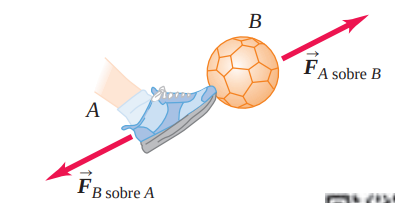
\includegraphics[width=0.5\linewidth]{figures/ac-reac.png}
    \end{figure}

    Dicho de otra forma, \begin{center}
    \textit{Si el cuerpo A ejerce una fuerza sobre
el cuerpo B (una “acción”), entonces, el cuerpo B ejerce una fuerza sobre el cuerpo A
(una “reacción”). Estas dos fuerzas tienen la misma magnitud pero dirección opuesta,
y actúan sobre cuerpos diferentes.}
\end{center}

    Si un cuerpo aislado sufre una aceleraci\'on y no podemos encontrar un objeto externo que sufre una aceleraci\'on igual pero opuesta, entonces estaremos en problemas. Un ejemplo mas típico de un par acción-reacción es el de dos patinadores sobre hielo intercambiando una pelota.
\end{frame}

\begin{frame}{Ejercicio}

Dos adultos y un ni\~no quieren empujar un carrito con ruedas en la direcci\'on $x$ como se ilustra en la figura. 
Los adultos empujan con fuerzas horizontales $F_1$ y $F_2$ como se muestra en la figura. 

\begin{enumerate}
    \item[(a)] Calcule la magnitud y direcci\'on de la fuerza \textit{m\'as peque\~na} que el ni\~no debe ejercer. Se pueden despreciar los efectos de la fricci\'on.
    \item[(b)] Si el ni\~no ejerce la fuerza m\'inima obtenida en el inciso (a), el carrito acelerar\'a a $2.0\,\unit{m/s^2}$ en la direcci\'on $+x$. \\
    \textquestiondown Cu\'anto pesa el carrito?
\end{enumerate}

\begin{figure}
    \centering
    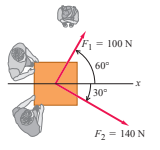
\includegraphics[width=0.3\linewidth]{figures/p1newton.png}
\end{figure}
    
\end{frame}

\begin{frame}{Resumen}
    \begin{align}
        \sum_i \vec{F}_i&=\vec{0}\quad\Rightarrow\quad \text{Primera ley de Newton}\,,\\
        \sum_i \vec{F}_i&=m\vec{a}\quad\Rightarrow\quad \text{Segunda ley de Newton}\,,\\
        \vec{F}_{1\rightarrow2}&=-\vec{F}_{2\rightarrow1}\quad\Rightarrow\quad \text{Tercera ley de Newton}\,,\\
        \vec{w}&=m\vec{g}\quad\Rightarrow\quad \text{Fuerza gravitacional (peso)}\,.
    \end{align}
\end{frame}

\begin{frame}
    \begin{figure}
        \centering
        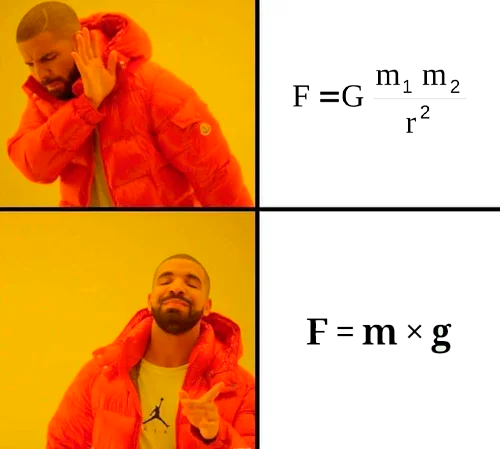
\includegraphics[width=0.5\linewidth]{figures/fgrav-meme.png}
    \end{figure}
\end{frame}

\begin{frame}
    \begin{figure}
        \centering
        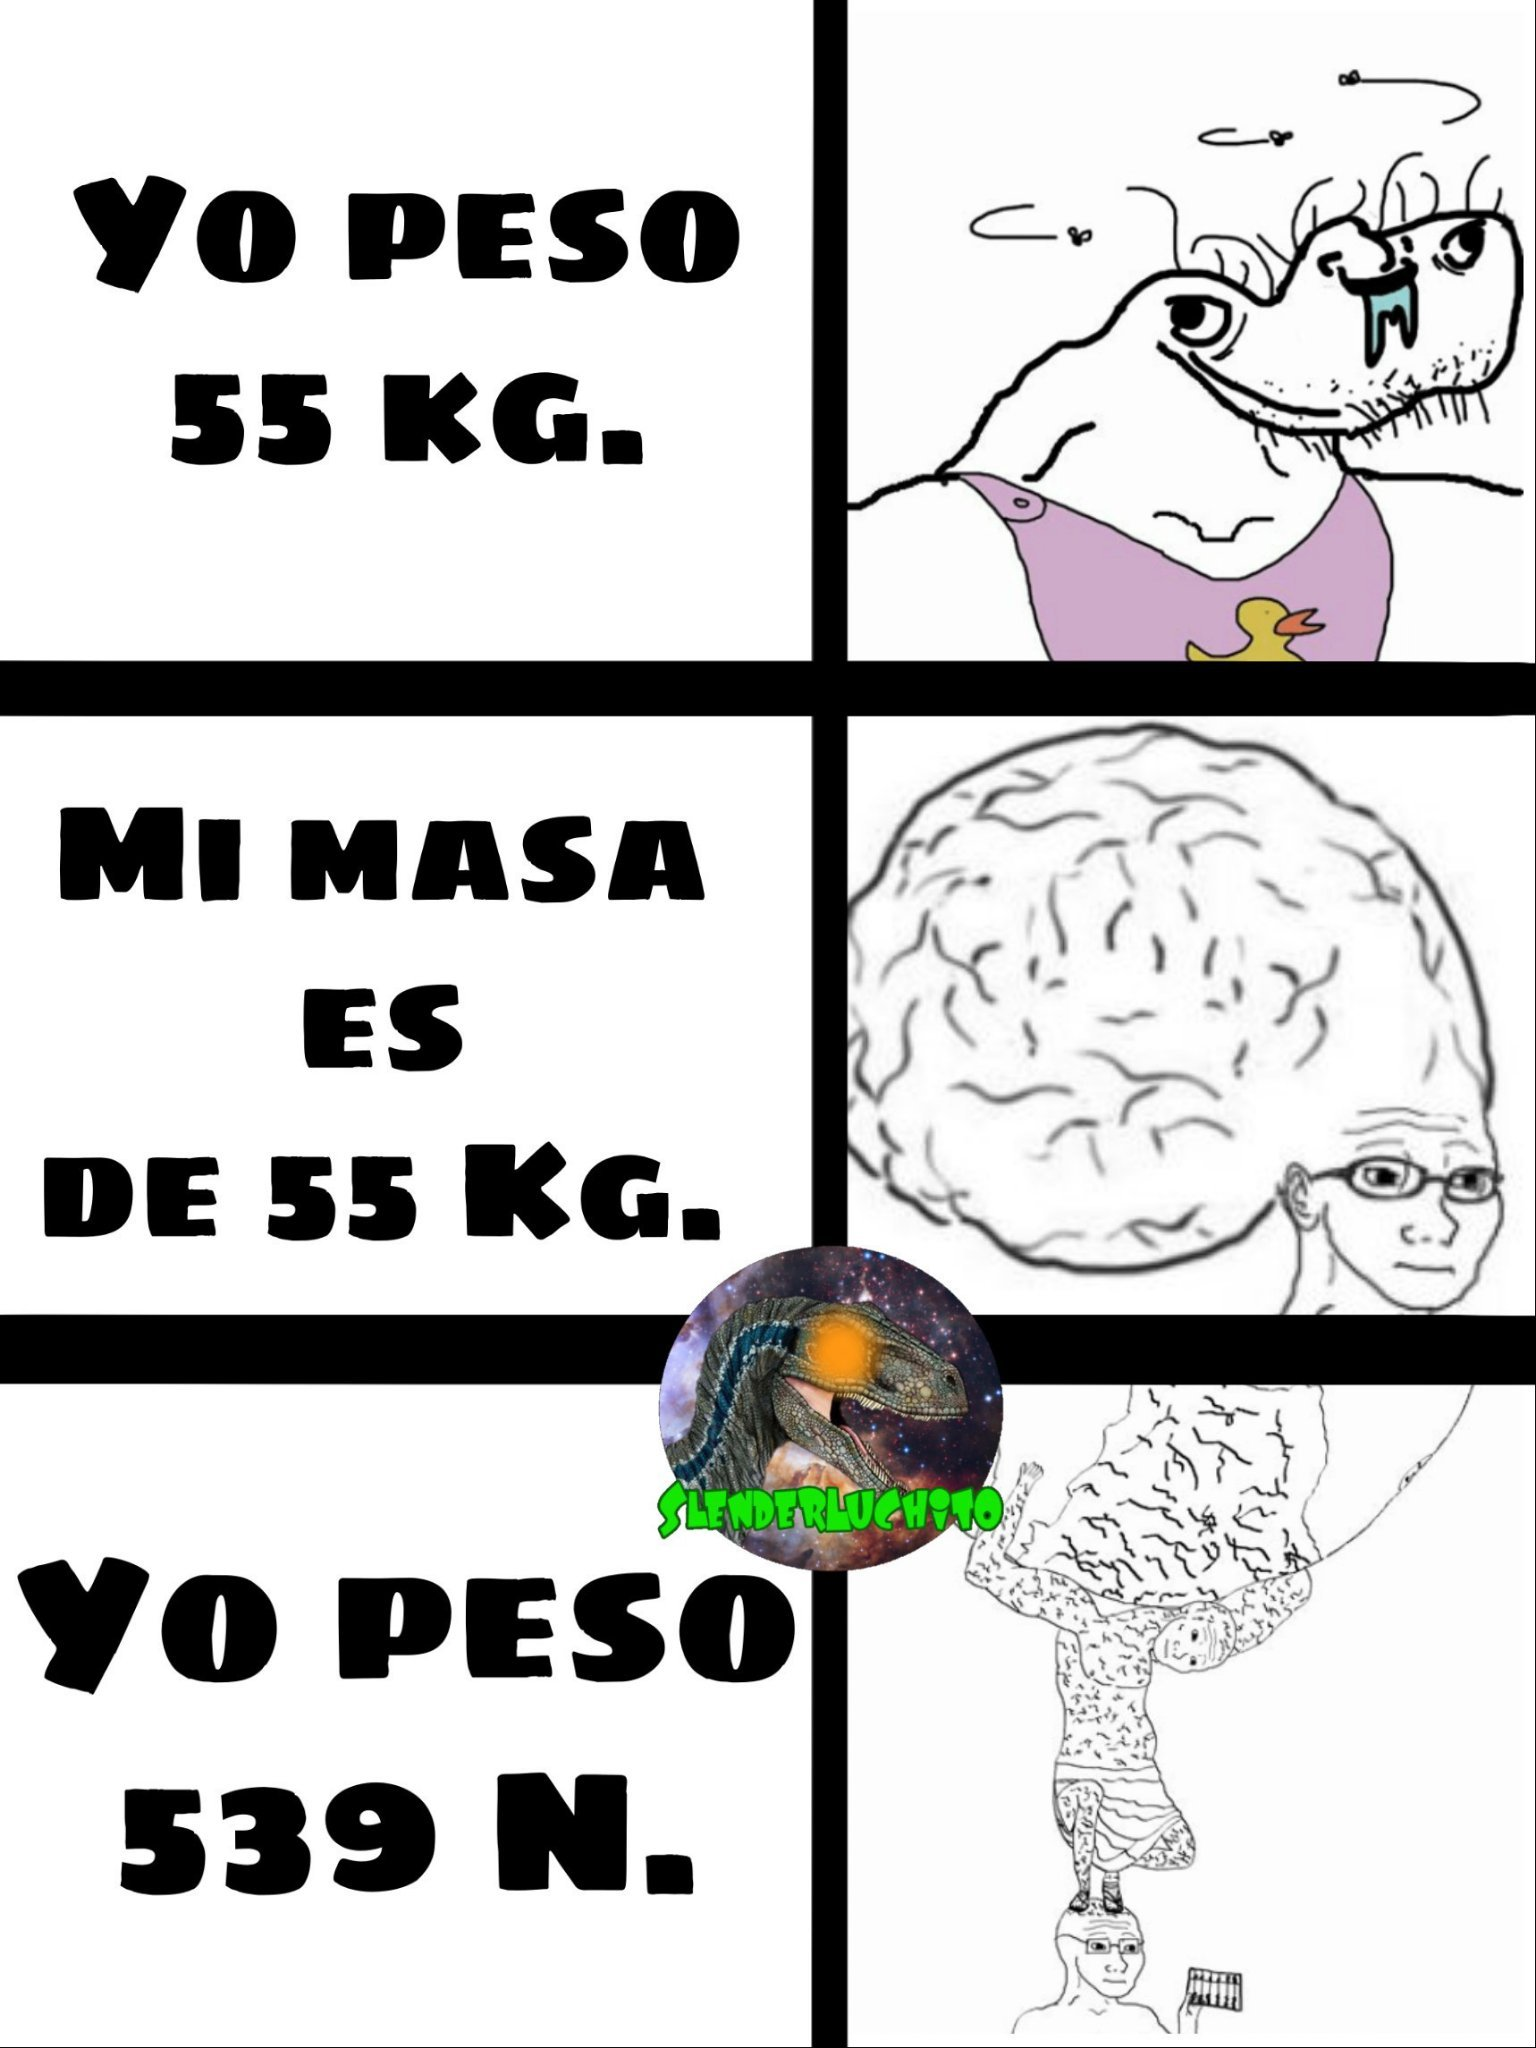
\includegraphics[width=0.5\linewidth]{figures/peso-meme.png}
    \end{figure}
\end{frame}

\begin{frame}{Diagramas de cuerpo libre}
    Un Diagrama de Cuerpo Libre (DCL) es una representación geométrica de los vectores de fuerza que actúan sobre un sistema. Las fuerzas son vectores libres que, en el caso ideal, actúan sobre el mismo lugar geométrico del sistema: el centro de masa (c.d.m.).
\end{frame}

\begin{frame}
    \begin{center}
        \Huge Veamos muchos ejemplos
    \end{center}
\end{frame}

\begin{frame}
\begin{columns}
\column{0.45\textwidth}
    \begin{figure}
        \centering
        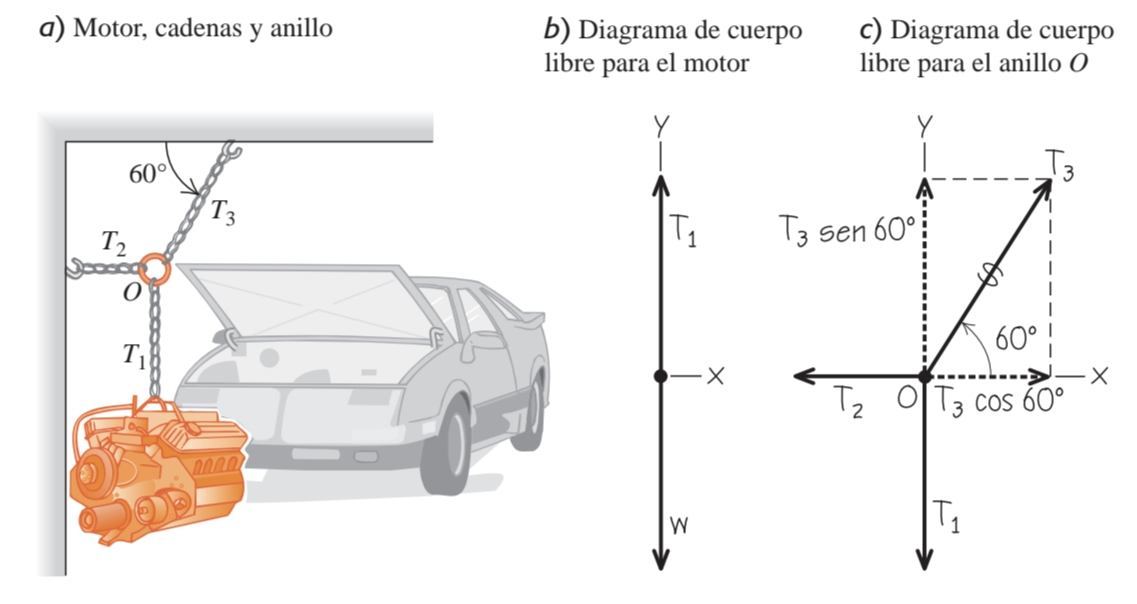
\includegraphics[width=1\linewidth]{figures/diagrama1.jpg}
    \end{figure}

\column{0.45\textwidth}
    \begin{figure}
        \centering
        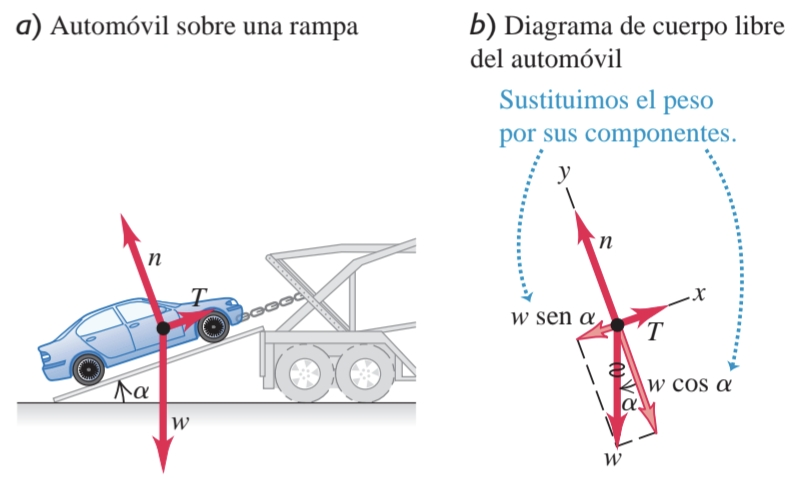
\includegraphics[width=1\linewidth]{figures/diagrama2.jpg}
    \end{figure}
\end{columns}

\begin{columns}
\column{0.45\textwidth}
    \begin{figure}
        \centering
        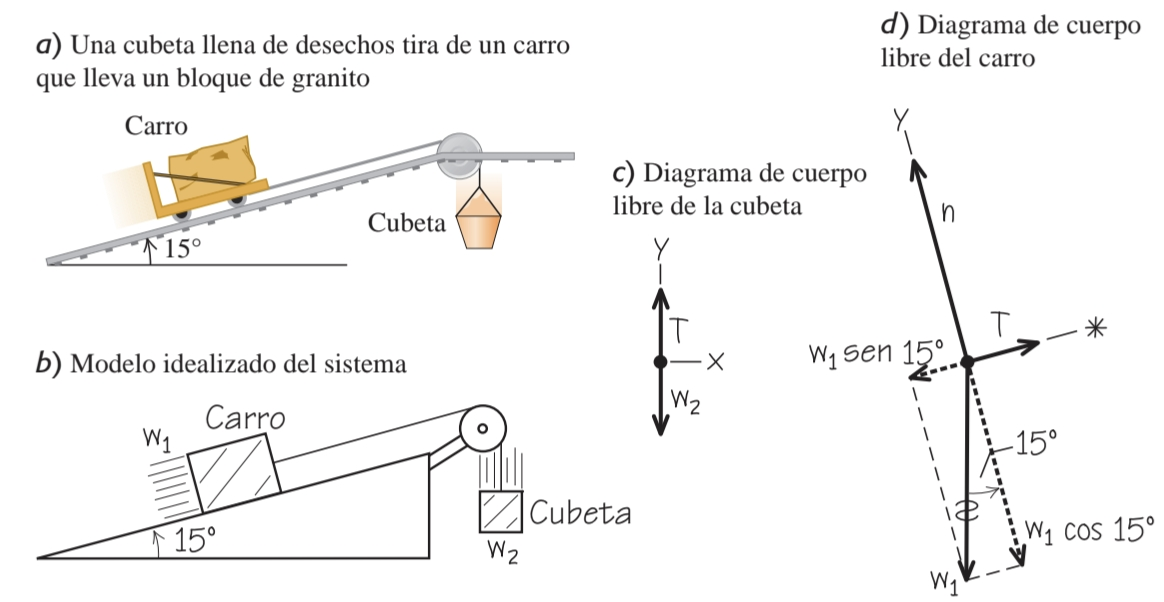
\includegraphics[width=1\linewidth]{figures/diagrama3.jpg}
    \end{figure}

\column{0.45\textwidth}
    \begin{figure}
        \centering
        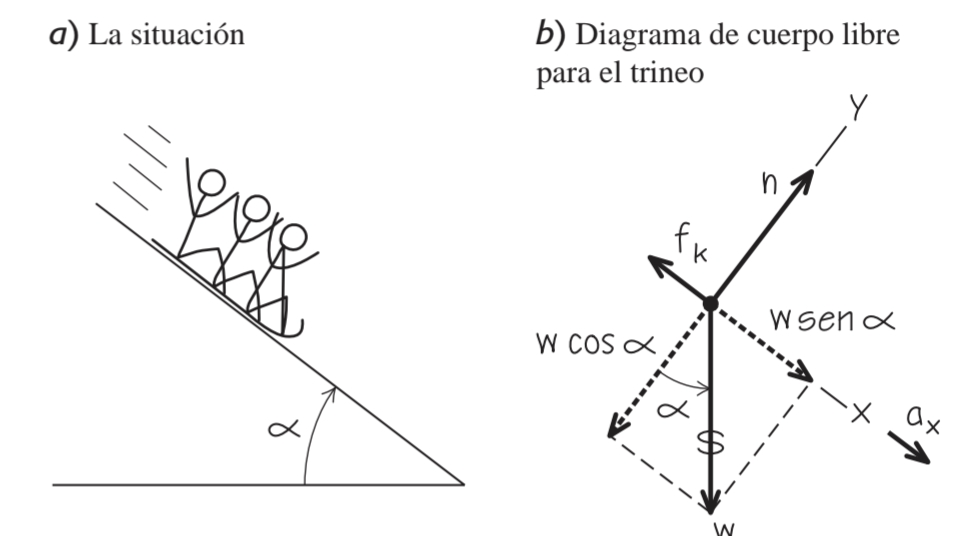
\includegraphics[width=1\linewidth]{figures/diagrama4.jpg}
    \end{figure}
\end{columns}
    
\end{frame}

\begin{frame}
\begin{columns}
\column{0.45\textwidth}
    \begin{figure}
        \centering
        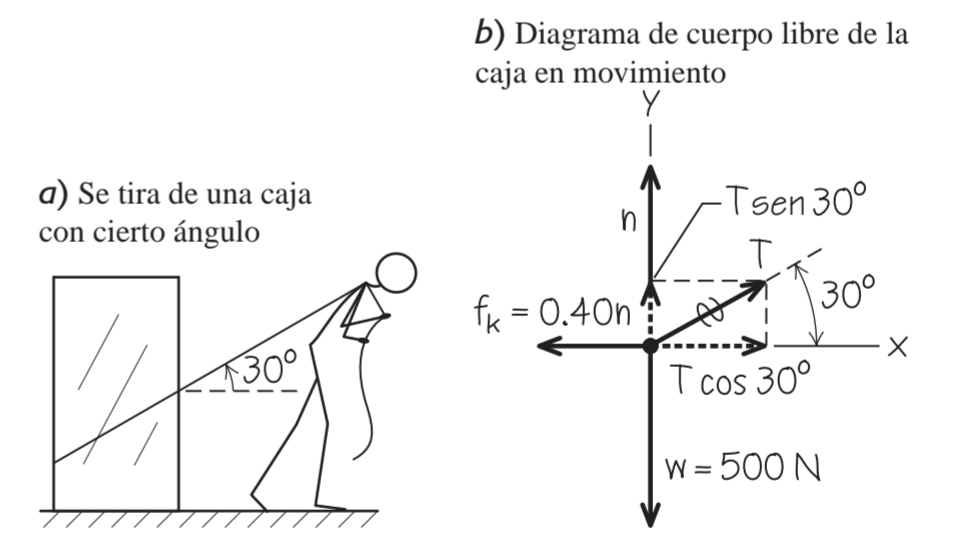
\includegraphics[width=1\linewidth]{figures/diagrama5.jpg}
    \end{figure}

\column{0.45\textwidth}
    \begin{figure}
        \centering
        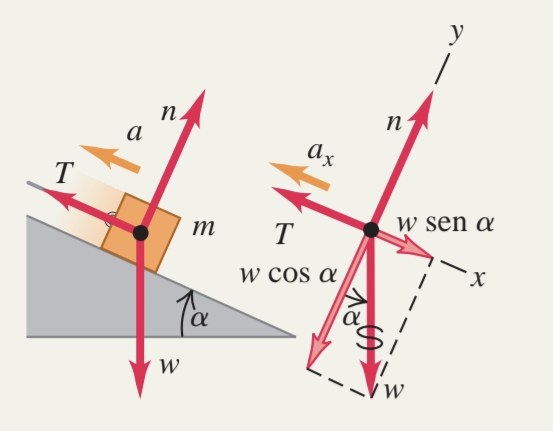
\includegraphics[width=1\linewidth]{figures/diagrama6.jpg}
    \end{figure}
\end{columns}
    
\end{frame}

\begin{frame}
\begin{columns}
\column{0.45\textwidth}
    \begin{figure}
        \centering
        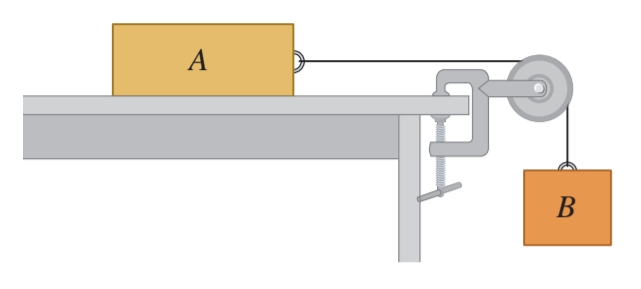
\includegraphics[width=1\linewidth]{figures/poleas1.jpg}
    \end{figure}

\column{0.45\textwidth}
    \begin{figure}
        \centering
        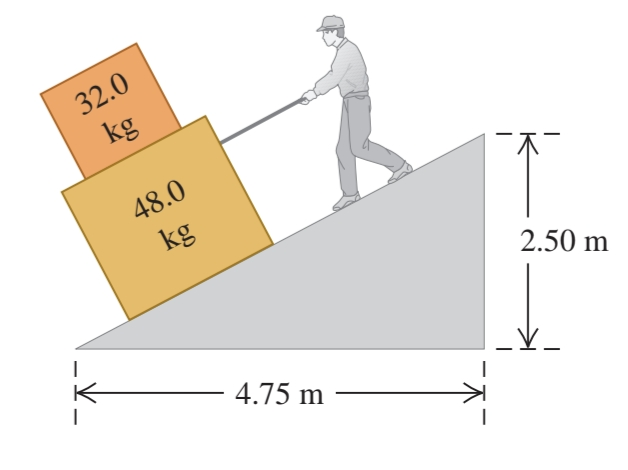
\includegraphics[width=1\linewidth]{figures/cajas1.jpg}
    \end{figure}
\end{columns}
    
\end{frame}

\begin{frame}
\begin{columns}
\column{0.45\textwidth}
    \begin{figure}
        \centering
        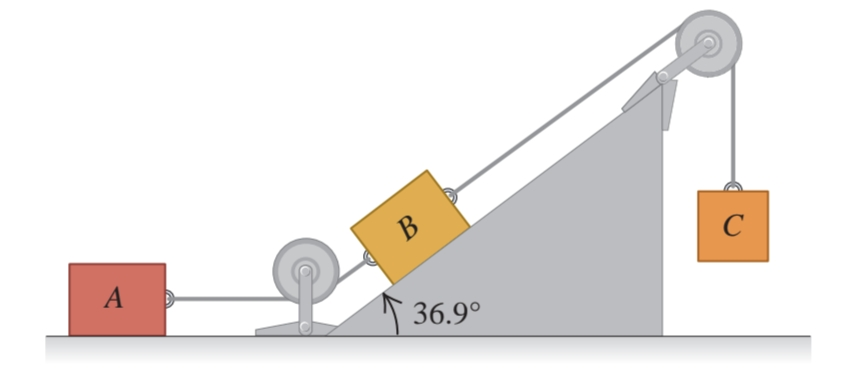
\includegraphics[width=1\linewidth]{figures/poleas-y-cajas1.jpg}
    \end{figure}

\column{0.45\textwidth}
    \begin{figure}
        \centering
        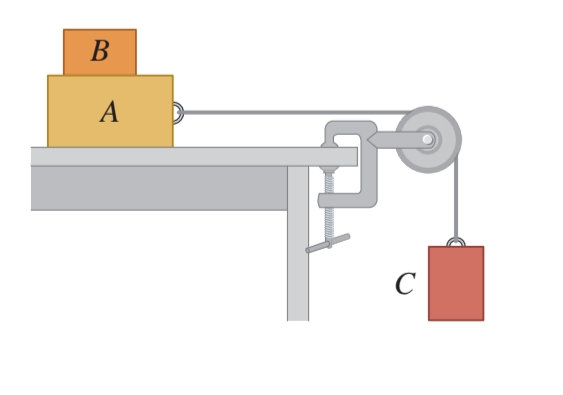
\includegraphics[width=1\linewidth]{figures/cajas2.jpg}
    \end{figure}
\end{columns}
    
\end{frame}

\begin{frame}
    \begin{center}
        \Huge ¿Preguntas?
    \end{center}
\end{frame}

\begin{frame}
    \begin{center}
        \LARGE \textbf{Fuerzas de fricción}
    \end{center}
\end{frame}

\begin{frame}{Fuerzas de contacto}
    Siempre que dos cuerpos interactúan por contacto directo de sus superficies (se tocan), describimos la interacción en términos de fuerzas de contacto.
    \vspace{1em}
    
    \begin{columns}
        \column{0.45\textwidth}
        \textbf{Fuerzas superficiales o de contacto}
        \vspace{1em}
        \begin{itemize}
            \item Tensión
            \item Normal
            \item Empuje
            \item Fricción

            $\vdots$
        \end{itemize}
        \column{0.45\textwidth}
        \textbf{Fuerzas másicas o volumétricas}
        \vspace{1em}

        \begin{itemize}
            \item Gravitacional
            \item Eléctrica
            \item Magnética
            \item Nuclear

            $\vdots$
        \end{itemize}
        
    \end{columns}
\end{frame}

\begin{frame}{Fuerza de fricción}

La fuerza de fricción es una fuerza que se opone al movimiento relativo (o a la tendencia de movimiento) entre dos superficies que están en contacto.

En otras palabras, cuando un objeto intenta deslizarse o moverse sobre otro, aparece una fuerza que actúa en dirección contraria al movimiento o intento de movimiento, y esa fuerza es la fricción.
    
\end{frame}

\begin{frame}{Tipos de fuerza de fricción}

    \textbf{Fricción estática} (\( f_s \))
    \begin{itemize}
        \item Actúa cuando el objeto está \textbf{en reposo} respecto a la superficie.
        \item Evita que el objeto comience a moverse.
        \item Aumenta conforme aplicas más fuerza, hasta un \textbf{valor máximo}.
        \item Se cumple:
        \[
        f_s \leq \mu_s \, N
        \]
        donde \(\mu_s\) es el coeficiente de fricción estática y \(N\) es la fuerza normal (la fuerza que ejerce la superficie sobre el objeto perpendicularmente a ella).
    \end{itemize}
    \end{frame}

    \begin{frame}
        \textbf{Fricción cinética o dinámica} (\( f_k \))
    \begin{itemize}
        \item Actúa cuando el objeto está \textbf{en movimiento} sobre la superficie.
        \item Tiene un \textbf{valor constante} (menor que el máximo de la fricción estática).
        \item Se calcula como:
        \[
        f_k = \mu_k \, N
        \]
        donde \(\mu_k\) es el coeficiente de fricción cinética.
    \end{itemize}
    \end{frame}

\begin{frame}{Comportamiento}
    \begin{figure}
        \centering
        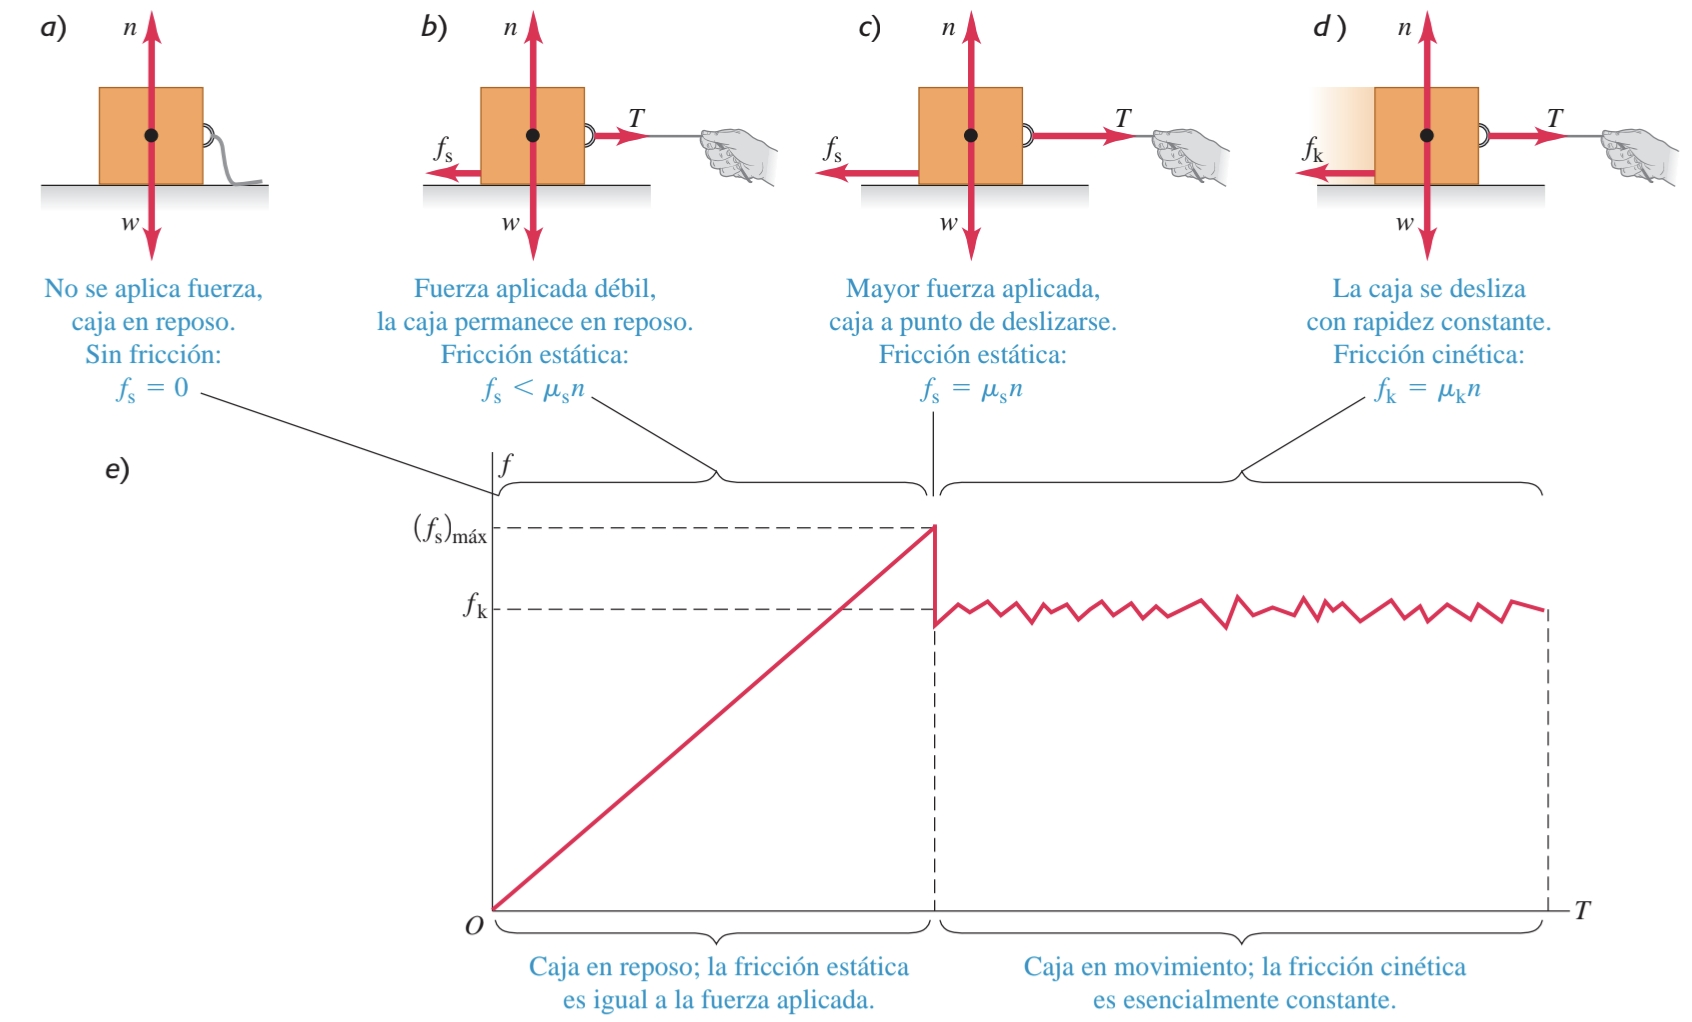
\includegraphics[width=1\linewidth]{figures/friccion.jpg}
    \end{figure}
\end{frame}

\begin{frame}{Factores que afectan la fricción}

\begin{itemize}
    \item \textbf{Naturaleza de las superficies}: rugosas $\rightarrow$ más fricción, lisas $\rightarrow$ menos fricción.
    \item \textbf{Fuerza normal \(N\)}: a mayor fuerza que presione las superficies entre sí, mayor será la fricción.
    \item \textbf{Estado del movimiento}: reposo o movimiento.
\end{itemize}

\vspace{1em}

\textbf{Importancia de la fricción}

\begin{itemize}
    \item Permite \textbf{caminar y frenar} (sin fricción los pies resbalarían).
    \item Es necesaria para que \textbf{los vehículos avancen o frenen}.
    \item También puede ser una \textbf{resistencia indeseada} (en máquinas, motores, rodamientos).
\end{itemize}

\end{frame}

\begin{frame}{Coeficientes de fricción}
    \begin{figure}
        \centering
        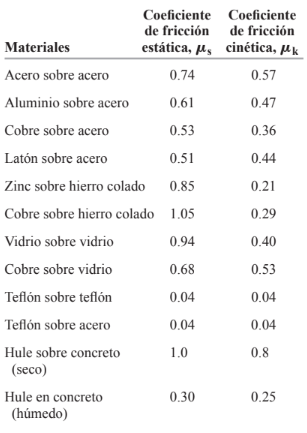
\includegraphics[width=0.4\linewidth]{figures/coef-fric.png}
    \end{figure}
\end{frame}

\begin{frame}{Ejemplo}
    Una caja de bananas que pesa 40.0 N descansa en una superficie horizontal. El coeficiente de fricción estática entre la caja y la
superficie es de 0.40, y el coeficiente de fricción cinética es de 0.20.
\begin{itemize}
    \item[a)] Si no se aplica alguna fuerza horizontal a la caja en reposo, ¿qué tan grande es la fuerza de fricción ejercida sobre la caja?
    \item[b)] ¿Qué magnitud tiene la fuerza de fricción si un mono aplica una fuerza horizontal de 6.0 N a la caja inicialmente en reposo?
    \item[c)] ¿Qué fuerza horizontal mínima debe aplicar el mono para poner en movimiento la caja?
    \item[d)] ¿Qué fuerza horizontal mínima debe aplicar el mono para que la
caja siga moviéndose con velocidad constante, una vez que haya comenzado a moverse?
\item[e)] Si el mono aplica una fuerza horizontal de 18.0 N, ¿qué magnitud tiene la fuerza de fricción y qué aceleración
tiene la caja?
\end{itemize}

\end{frame}

\begin{frame}{Fuerza viscosa}

La \textbf{fuerza viscosa} es la \textbf{resistencia que ofrece un fluido (líquido o gas) al movimiento de un objeto que se desplaza a través de él}.  
Esta fuerza surge por la \textbf{viscosidad} del fluido, que es una medida de su \textbf{resistencia interna al flujo}.

\begin{itemize}
    \item Siempre actúa en dirección \textbf{opuesta al movimiento} del objeto.
    \item Depende de:
    \begin{itemize}
        \item la \textbf{velocidad} del objeto,
        \item la \textbf{forma y tamaño} del objeto,
        \item y la \textbf{viscosidad del fluido}.
    \end{itemize}
    \item Es un tipo de \textbf{fuerza de fricción}, pero que aparece cuando hay \textbf{interacción con un fluido} (aire, agua, aceite, etc.).
\end{itemize}

\end{frame}

\begin{frame}{Ley de Stokes}

Para flujo laminar y objetos esféricos pequeños con velocidades bajas, la fuerza viscosa se puede calcular con la ley de Stokes:

\[
f = 6 \pi \, \eta \, r \, v
\]

donde:
\begin{itemize}
    \item \(\eta\): viscosidad del fluido,
    \item \(r\): radio de la esfera,
    \item \(v\): velocidad del objeto en el fluido.
\end{itemize}

\end{frame}

\begin{frame}{Velocidades y fuerza viscosa}
    En general, para velocidades pequeñas, \begin{equation}
        f\propto v\,,
    \end{equation} y a altas velocidades, \begin{equation}
        f\propto v^2\,.
    \end{equation}
\end{frame}

\begin{frame}{Ecuaciones de movimiento}
    Para un objeto de masa $m$ que cae en el seno de un fluido viscoso de resistencia $k$ pequeñas velocidades, la ecuación de movimiento está dada por \begin{equation}
        m\frac{dv}{dt}=mg-kv\,.
    \end{equation} En un sistema de referencia en el que $(y_0,v_0,t_0)=(0,0,0)$, la solución a esta ecuación diferencial ordinaria es \begin{align}
        a(t)&=ge^{-\frac{g}{v_t}t}\,,\\
        v(t)&= v_t\left(1-e^{-\frac{g}{v_t}t}\right)\,,\\
        y(t)&=v_tt-\frac{v_t^2}{g}\left(1-e^{-\frac{g}{v_t}t}\right)\,,
    \end{align} donde $v_t=mg/k$ se define como la velocidad terminal del sistema.
\end{frame}

\begin{frame}{Evolución}
    \begin{figure}
        \centering
        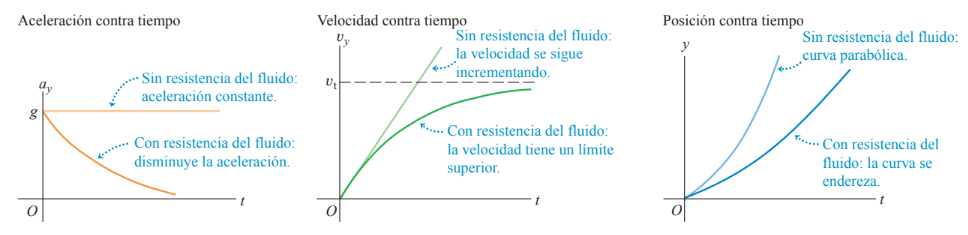
\includegraphics[width=1\linewidth]{figures/vel-terminal.png}
    \end{figure}
\end{frame}

\begin{frame}
    \begin{center}
        \Huge \textbf{Dinámica del movimiento circular}
    \end{center}
\end{frame}

\begin{frame}{Aceleración centrípeta}
    Cuando una partícula describe una circunferencia con rapidez constante, su aceleración siempre es hacia el centro de la circunferencia (perpendicular a la velocidad instantánea). La magnitud $a_c$ de la aceleración es constante y está dada en términos de la rapidez $v$ y el radio $r$ de la circunferencia por \begin{equation}
        a_c = \frac{v^2}{r}=\omega^2r=\frac{4\pi^2r}{T^2}=4\pi^2rf^2
    \end{equation}

    La fuerza central responsable del movimiento circular es conocida como \textit{fuerza centrípeta} $\vec{F}_c$. De acuerdo con Newton, \begin{equation}
        F_c = ma_c
    \end{equation}
\end{frame}

\begin{frame}
\begin{columns}
    \column{0.45\textwidth}
    \begin{figure}
        \centering
        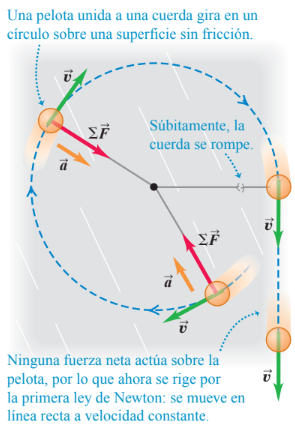
\includegraphics[width=\linewidth]{figures/Fcpta.png}
    \end{figure}
    \column{0.45\textwidth}
    \begin{figure}
        \centering
        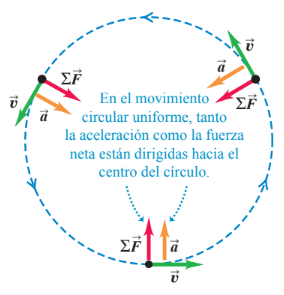
\includegraphics[width=\linewidth]{figures/acepta.png}
    \end{figure}
\end{columns}
\end{frame}

\begin{frame}{Ejemplo}
    El automóvil deportivo de la figura recorre una
curva de radio $R$. Si el coeficiente de fricción
estática entre los neumáticos y la carretera es $\mu_s$, ¿cuál es la rapidez
máxima con que el conductor puede tomar la curva sin derrapar?

\begin{figure}
    \centering
    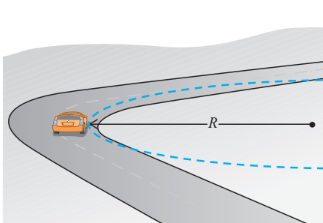
\includegraphics[width=0.45\linewidth]{figures/sin-peralte.png}
\end{figure}

\end{frame}

\begin{frame}{Ejemplo}
    Para un automóvil que viaja con cierta rapidez, es posible peraltar una curva con un ángulo tal que el automóvil no necesite fricción para mantener el radio con que da vuelta. Entonces el automóvil podría tomar con seguridad la curva aun sobre hielo húmedo. (Las carreras de trineos se basan en la misma idea). Un ingeniero propone reconstruir la curva
del ejemplo anterior de modo que un automóvil con rapidez $v$ pueda dar la
vuelta sin peligro aunque no haya fricción. ¿Qué ángulo
de peralte $\beta$ debería tener la curva?

\begin{figure}
    \centering
    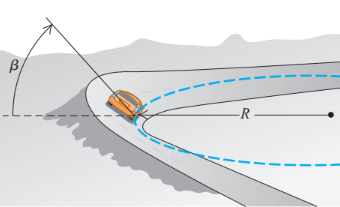
\includegraphics[width=0.45\linewidth]{figures/con-peralte.png}
\end{figure}

\end{frame}

\begin{frame}{Ejercicio}
    Un bloque pequeño de masa $m$ se coloca dentro de un cono invertido que gira sobre un eje vertical, de modo que la duración de una revolución del cono es $T$. La pared del cono forma un ángulo $\beta$ con la horizontal. El coeficiente de fricción estática entre el bloque y el cono es $\mu_s$. Si el bloque debe mantenerse a una altura constante $h$ sobre el vértice del cono,
    \begin{itemize}
        \item[a)] ¿Cuál es el valor máximo de $T$?
        \item[b)] ¿el valor mínimo de $T$?
    \end{itemize}

    \begin{figure}
        \centering
        \includegraphics[width=0.35\linewidth]{figures/cono-rev.png}
    \end{figure}
    
\end{frame}

\begin{frame}{Ejercicio}
    El bloque de 4.00 kg
de la figura está sujeto a
una varilla vertical con dos cuerdas. Cuando el sistema gira en
torno al eje de la varilla, las cuerdas se extienden como se indica
en el diagrama, y la tensión en
la cuerda superior es de 80.0 N.

\begin{figure}
    \centering
    \includegraphics[width=0.25\linewidth]{figures/dos-cuerdas.png}
\end{figure}

\begin{itemize}
    \item[a)] ¿Qué tensión hay en la cuerda
inferior?
\item[b)] ¿Cuántas revoluciones por minuto realiza el sistema?
\item[c)] Calcule las revoluciones por minuto con las que la cuerda inferior pierde su tensión. 
\item[d)] Explique qué sucede si el número de rpm es menor que en el inciso c).
\end{itemize}

\end{frame}

\begin{frame}{Ejercicio}
    El “columpio gigante” de una feria local consiste en un eje vertical central con varios brazos horizontales unidos a su extremo superior. Cada brazo sostiene un asiento suspendido
de un cable de 5.00 m, sujeto al brazo en un punto a 3.00 m del eje
central.

\begin{figure}
    \centering
    \includegraphics[width=0.35\linewidth]{figures/juego-feria.png}
\end{figure}

\begin{itemize}
    \item[a)] Calcule el tiempo de una revolución del columpio, si el
cable forma un ángulo de 30.0° con la vertical.
    \item[b)] ¿El ángulo depende
del peso del pasajero para una velocidad de giro determinada?
\end{itemize}
\end{frame}

\begin{frame}
    \begin{center}
        \Huge Hagamos un experimento teórico
    \end{center}
\end{frame}

\begin{frame}
    \begin{figure}
        \centering
        \includegraphics[width=0.8\linewidth]{figures/exp-teo1.png}
    \end{figure}

    \begin{center}
        \large ¿Qué es $Fd$?
    \end{center}

    \pause \begin{center}
        \LARGE NADA.
    \end{center}
    
\end{frame}

\begin{frame}
    \begin{figure}
        \centering
        \includegraphics[width=0.8\linewidth]{figures/exp-teo2.png}
    \end{figure}

    \begin{center}
        \large Y aquí... ¿Qué es $Fd$?
    \end{center}

    \pause \begin{center}
        \LARGE NADA.
    \end{center}

    \pause \begin{center}
        \large ¿Pero qué es $(F\cos\theta)d$?
    \end{center}
    
    
\end{frame}

\begin{frame}
    \begin{center}
        Ah, pero $(F\cos\theta)d$ es...
    \end{center}

    \begin{center}
        \pause \Large $\vec{F}\cdot\vec{r}$
        
        \pause \large ¿Y eso qué es?
        
        \vspace{2em} \pause \Huge NADA.
    \end{center}
\end{frame}

\begin{frame}
\begin{center}
    ¿Y si el suelo es curvo?
    
    \pause Pues...

    \begin{equation*}
        \int_c\vec{F}\cdot d\vec{r}
    \end{equation*}

    \pause ¿Y si la fuerza no es constante ?
    
    \pause Pues...

    \begin{equation*}
        \int_c\vec{F}(\vec{r},\vec{v},t)\cdot d\vec{r}
    \end{equation*}

    \end{center}
    
\end{frame}

\begin{frame}
    \begin{figure}
        \centering
        \includegraphics[width=0.4\linewidth]{figures/meme-que-es.png}
    \end{figure}
    
    \begin{center}
        \vspace{3em} \pause \Huge \textbf{NADA.}
    \end{center}
\end{frame}

\begin{frame}
\begin{center}
    Bueno ya, pongámonos serios...

    \vspace{4em}
    \pause El trabajo se define como \begin{equation*}
        W=\int_c\vec{F}(\vec{r},\vec{v},t)\cdot d\vec{r}
    \end{equation*}


\pause ¿Eso así pa' qué?

\vspace{2em}

\pause     \Huge \textbf{Pa' NADA.}
\end{center}
    
\end{frame}

\begin{frame}
    \begin{center}
        \Huge ¿O...?
    \end{center}
\end{frame}

\begin{frame}{Ejemplo}
    \begin{figure}
        \centering
        \includegraphics[width=0.4\linewidth]{figures/ejmeplo-trabajo1.png}
    \end{figure}
\end{frame}

\begin{frame}
    Considere el sistema de la
figura. La cuerda y la polea
tienen masas despreciables, y la
polea no tiene fricción. Entre el
bloque de 8 kg y la mesa,
el coeficiente de fricción cinética
es 0.25. Los bloques se
sueltan del reposo. Determine el trabajo efectúa \begin{itemize}
    \item[a)] sobre el bloque de 6 kg \begin{itemize}
        \item[\textit{i}.] la gravedad y
        \item[\textit{ii}.] la tensión en el cordón.
    \end{itemize}
    \item[b)] sobre el bloque de 8 kg \begin{itemize}
        \item[\textit{i}.] la gravedad,
        \item[\textit{ii}.] tensión en el cordón,
        \item[\textit{iii}.] la fricción y
        \item[\textit{iv}.] la fuerza normal
    \end{itemize}
    \item[c)] Obtenga el trabajo total efectuado sobre cada bloque.
    \item[d)] Obtenga el trabajo total efectuado sobre el sistema.
    \item[e)] Use métodos de energía para calcular la rapidez del bloque de 6 kg después de descender 1.5 m.
\end{itemize}, 



\end{frame}
    
    \begin{frame}{Resultados de la sesión anterior}
        
    \begin{itemize}
        \pause \item El trabajo es el acto de transformar la materia aplicando fuerzas (Maxwell, 1877).
        En general,
        
        \pause $$W=\int_l \Vec{F}\cdot d\Vec{r}.$$
        
        \pause \item La energía es la capacidad que tiene un sistema de generar transformaciones (Domenech et al, 2003)
        
        \pause \item La energía se clasifica en dos tipos:
        \vspace{0.5em}
        
        \begin{columns}
            \column[t]{6cm}
            \centering
            \pause \textbf{Energía cinética}
            
            \begin{equation}
            \pause     K=\frac{1}{2}mv^2.
            \end{equation}
            
            \column[t]{6cm}
            \centering
            \pause \textbf{Energías potenciales}
            \begin{equation}
             \pause    U_g=mgy,
            \end{equation}
            
            \begin{equation}
             \pause    U_E=\frac{1}{2}kx^2.
            \end{equation}
            
        \end{columns}
    \end{itemize}
        
    \end{frame}
    
%%%%%%%%%%%%%%%%%%%%%%%%%%%%%%%%%%%%%%%%%%   DIAPOSITIVA 2
    
    \begin{frame}{Teoremas del trabajo y la energía}
        \begin{itemize}
            \pause \item La energía cinética es dependiente de la velocidad de la partícula.
            
            \pause \item La energía potencial es dependiente de la posición de la partícula.
            
            \pause \item Existen relaciones entre el trabajo y la energía asociada a un sistema.
            
            \begin{equation}
             \pause    W=\Delta K,
            \end{equation}
            
            \begin{equation}
             \pause    W_g=-\Delta U_g,
            \end{equation}
            
            \begin{equation}
             \pause    W_E=-\Delta U_E.
            \end{equation}
            
        \end{itemize}
        
    \end{frame}
    
%%%%%%%%%%%%%%%%%%%%%%%%%%%%%%%%%%%%%%%%%%   DIAPOSITIVA 3
    
    \begin{frame}{Fuerzas conservativas}
    
        \begin{itemize}
        \pause \item Se dice que una fuerza es conservativa, si el trabajo que desarrolla dicha fuerza para mover un objeto de un punto $A$ a un punto $B$, es independiente de la trayectoria.
        
        \begin{figure}
            \centering
            \includegraphics[scale=0.3]{figures/FNC.png}
        \end{figure}
        
        \pause \item Por ejemplo, la fuerza de atracción gravitacional es una fuerza conservativa, al igual que la fuerza de Hooke.
        
        \begin{figure}
            \centering
            \includegraphics[scale=1.3]{figures/FCONS.png}
        \end{figure}
        \end{itemize}
        
    \end{frame}
    
    \begin{frame}{Propiedades de las fuerzas conservativas}
    
        \begin{itemize}
        \pause \item Toda fuerza conservativa, que almacena una energía potencial $U$ en el sistema, verifica la relación
        
        \pause \begin{equation}
             F^{\text{ctva}}=-\frac{dU}{dr}.
        \end{equation}
        
        \pause \item El trabajo desarrollado por una fuerza conservativa en una trayectoria cerrada es \textit{nulo}, es decir,
        
        \begin{equation}
        \pause     W=\oint_c \vec{F}^{\text{ctva}}\cdot d\vec{r}=0.
        \end{equation}
        
        \pause \item La noción cualitativa de \textit{fuerza conservativa} es un tipo de fuerza que \textbf{conserva} la energía del sistema cuando desarrolla trabajo sobre él. No disipa la energía del sistema.
        
        \end{itemize}
        
    \end{frame}
    
%%%%%%%%%%%%%%%%%%%%%%%%%%%%%%%%%%%%%%%%%%   DIAPOSITIVA 5
    
    \begin{frame}{Fuerzas no conservativas}
        
        \begin{itemize}
            \pause \item Un fuerza es \textit{no conservativa}, si al desarrollar trabajo sobre un sistema, este pierde energía mecánica.
            
            \pause \item La fuerza de fricción es no conservativa
            
        \begin{figure}
            \centering
            \includegraphics[scale=0.7]{figures/FNOC.jpeg}
        \end{figure}
        
        \pause \item Las fuerzas no conservativas, transforman la energía del sistema en energía térmica a través del \textit{calor}, por esto, el sistema pierde energía y la cede al entorno. Así, el entorno adquiere energía térmica. 
        
        \end{itemize}
        
    \end{frame}
    
%%%%%%%%%%%%%%%%%%%%%%%%%%%%%%%%%%%%%%%%%%   DIAPOSITIVA 6
    
    \begin{frame}{Propiedades de la energía}
        
        \pause La naturaleza expone un comportamiento bastante interesante: la energía de un sistema
        
        \begin{enumerate}
            \pause \item Puede transferirse/transformar.
            
            \pause \item Se conserva.
            
            \pause \item Puede degradarse.
        \end{enumerate}
        
        \begin{columns}
            \column[t]{6cm}
            
            \pause \textbf{Mecanismos de transferencia de energía}
            
            \pause La energía puede transferirse a través de (entre otros),
            
            \begin{itemize}
                \pause \item Calor
                \pause \item Radicación electromagnética
                \pause \item Transmisión eléctrica
                \pause \item Transferencia de materia
                \pause \item Ondas mecánicas
            \end{itemize}
            
            \column[t]{6cm}
            
            \begin{figure}
            \centering
            \includegraphics[scale=0.2]{figures/Mecanismos.png}
            \end{figure}
            
            
        \end{columns}
        
\begin{columns}
    
\end{columns}
        
    \end{frame}
    
%%%%%%%%%%%%%%%%%%%%%%%%%%%%%%%%%%%%%%%%%%   DIAPOSITIVA 7
    
    \begin{frame}{Cambio en la energía total de un sistema \textit{no aislado}}
        
        \begin{itemize}
            \pause \item La energía se \textbf{transforma} en otros tipos de energía. Por ejemplo, al consumir alimentos, transformamos la energía química contenida en los elementos que consumimos, en energía cinética para movernos, y energía potencial para cambiar de posición en el espacio.
            
            \pause \item Todos los procesos en el acaecer del universo involucran transformaciones, intercambios y transferencia de energía.
            \pause \item El cambio en la energía total de un sistema, debido a la transferencia de energía del sistema a los alrededores, es tal que
            
            \begin{equation}
                \pause \underbrace{\Delta E_{\text{sistema}}=\sum E_{\text{transferidas al entorno}}}_{\text{sistema \textbf{no aislado}}}.
            \end{equation}
        \end{itemize}
        
        
    \end{frame}
    
%%%%%%%%%%%%%%%%%%%%%%%%%%%%%%%%%%%%%%%%%%   DIAPOSITIVA 8

    \begin{frame}{Cambio en la energía total de un sistema \textit{aislado}}
        \begin{columns}
            \column[t]{6cm}
            \pause En un sistema aislado, la energía \\ \textit{se conserva}, esto quiere decir que, el cambio en la energía  total del sistema es nulo. Es un invariante ante transformaciones temporales.
            
            \begin{equation}
            \pause     \Delta E_{\text{total}}=0.
            \end{equation}
            
            \pause La naturaleza expone este comportamiento, y desde hace mucho tiempo, los físicos lo han sabido, pero no fue hasta 1915 que la matemática alemana Emmy Noether, demostró que esto se debe gracias a la existencia de una simetría temporal
            
            \column[t]{6cm}
            y una invariancia del Lagrangiano de un sistema.
            
            \begin{figure}
            \centering
            \includegraphics[scale=0.13]{figures/Noether.jpg}
            \end{figure}

        \end{columns}
        
    \end{frame}
    
%%%%%%%%%%%%%%%%%%%%%%%%%%%%%%%%%%%%%%%%%%   DIAPOSITIVA 9

    \begin{frame}{Conservación de la energía}
        \begin{itemize}
            \pause \item La suma de todas las variaciones de energía de un sistema es idénticamente nula, esto es,
            
            \begin{equation}
            \pause     \Delta K+\Delta U_g + \Delta U_E=0.
            \end{equation}
            
            \pause \item Por ejemplo, un cuerpo que cae desde el reposo a una altura $h$, inicialmente, posee almacenada una energía potencial gravitacional $E_{\text{total}}=U_g^{\text{máx}}=mgh$. A medida que cae, su energía potencial se \textit{transforma} en energía cinética $K=mv^2/2$, pero en cada punto de la trayectoria donde posee energía potencial $U_g=mgy<mgh$, se verifica que
            
            \pause $$\frac{1}{2}mv^2+mgy=E_{\text{total}}=mgh=\text{constante}.$$
            
        \end{itemize}
    \end{frame}
    
%%%%%%%%%%%%%%%%%%%%%%%%%%%%%%%%%%%%%%%%%%   DIAPOSITIVA 10

    \begin{frame}{Ejemplo: conservación de la energía}
        \begin{figure}
            \centering
            \includegraphics[scale=0.5]{figures/Ejem.png}
        \end{figure}
    \end{frame}
    
%%%%%%%%%%%%%%%%%%%%%%%%%%%%%%%%%%%%%%%%%%   DIAPOSITIVA 11

    \begin{frame}{Degradación de la energía debido a fuerzas no conservativas}
        
        \begin{itemize}
            \pause \item Las fuerzas no conservativas disipan la energía de un sistema cuando efectúan trabajo sobre él. Es el caso de la fuerza de fricción cinética $f_k$.
            
            \pause \item El cambio entonces, de la energía de un sistema que posee fuerzas no conservativas actuando sobre él, viene dado por
            \begin{equation}
            \pause     \Delta E = -W_{\text{no-conservativas}}+{W}_{\text{otras-fuerzas}}.
            \end{equation}
            
            \pause \item Si se trata de las formas de energía estudiadas y de la fricción cinética, entonces, para el caso más simple,
            
            \begin{equation}
            \pause     \Delta K +\Delta U_g + \Delta U_E = -f_k d+{W}_{\text{otras-fuerzas}},
            \end{equation}
            
            \pause donde $d$ es la distancia recorrida por el sistema al experimentar la fuerza de fricción cinética.
            
        \end{itemize}
        
    \end{frame}
    
%%%%%%%%%%%%%%%%%%%%%%%%%%%%%%%%%%%%%%%%%%   DIAPOSITIVA 12

    \begin{frame}{Ejemplo: Energía de un sistema con fuerzas \textit{no conservativas}}
        
        Considérese un bloque de masa $m$ que se arrastra por la acción de una fuerza $\Vec{F}$, en un piso rugoso con coeficiente de fricción cinético $\mu_k$. La fuerza $\Vec{F}$ forma un ángulo $\theta$ con la horizontal y el cuerpo está inicialmente en reposo. ¿Cuál será la velocidad de dicho objeto cuando recorra una distancia $x$?
        
        \begin{figure}
            \centering
            \includegraphics[scale=0.5]{figures/Ejem2.png}
        \end{figure}
        
    \end{frame}
    
    \begin{frame}{Solución al planteamiento}
        
        \begin{columns}
            \column{.45\textwidth}
            
            \pause Al hacer un análisis de fuerzas en el cuerpo, se infiere la ecuación
            
            \pause $$N+F\sin\theta-mg=0,$$
            
            \pause luego,
            \begin{equation}
            \pause     N=mg-F\sin\theta
            \end{equation}.
        
            \pause El análisis de energía implica que
            
            \pause $$\Delta E = -W_{f_k}+W_{F},$$
            
            \column{.45\textwidth}
            
            \pause por tanto,
            
            \pause $$\Delta K=-f_k x+Fx\cos\theta,$$
            
            \begin{align*}
            \frac{1}{2}mv^2-\frac{1}{2}mv_0^2  = &
            \pause  &-\mu_kNx+Fx\cos\theta.
            \end{align*}
            
            
        \end{columns}
        
    \end{frame}
    
    \begin{frame}{Respuesta}
    
    \pause Se tiene $v_0=0$. Al despejar la expresión para $v$ en de esta última ecuación y sustituir la expresión de la fuerza normal anteriormente obtenida, se lee:
    
        \begin{equation}
        \pause     v=\sqrt{\frac{2x}{m}[(\cos\theta+\mu_k\sin\theta)F-\mu_kmg}]
        \end{equation}
    \end{frame}

    \begin{frame}{Ley de Hooke}
    \begin{block}{Enunciado}
        La \textbf{Ley de Hooke} establece que la deformación que experimenta un
        resorte u otro cuerpo elástico es proporcional a la fuerza aplicada, 
        siempre y cuando no se supere el límite elástico del material.
    \end{block}

    \vspace{0.3cm}

    \begin{block}{Expresión matemática}
        \[
            F_E = -k \Delta x\,
        \]
        donde:
        \begin{itemize}
            \item $F_E$ es la fuerza restauradora (N).
            \item $k$ es la constante de elasticidad del resorte (N/m).
            \item $\Delta x$ es la elongación o compresión respecto a la posición de equilibrio (m).
        \end{itemize}
    \end{block}

\end{frame}

\begin{frame}{Trabajo que efectúa la fuerza elástica}
    El trabajo que desarrolla la fuerza elástica sobre un sistema está dado por \begin{equation}
        W_E=\Delta U_E\,,
    \end{equation} Donde \begin{equation}
        W_E=\frac{1}{2}k x^2\,.
    \end{equation}
\end{frame}

\begin{frame}{Comportamiento}
    \begin{figure}
        \centering
        \includegraphics[width=0.5\linewidth]{figures/hooke-law.png}
    \end{figure}
\end{frame}

\begin{frame}{Ejercicio}
        Un bloque de 200 g permanece en reposo en A cuando el muelle de constante 500 N/m está comprimido 7.5 cm. Se suelta el dispositivo de sujeción y el bloque recorre el camino ABCD. Calcular la velocidad del bloque en los puntos B, C y D.
        %considerando $\mu_k^{\arc{\text{ABC}}}=0.1$
        \begin{figure}
            \centering
            \includegraphics[width=0.25\linewidth]{figures/resorte-curva1.png}
        \end{figure}
    \end{frame}


    \begin{frame}{Ejercicio}
    Desde la ventana de un edificio de 15 m de altura se lanza un objeto de masa $m = 400$ g hacia la calle, utilizando un resorte con una constante de elasticidad de 750  N/m, como muestra la figura. El objeto a una distancia inicial de 80 cm se desplaza 10 cm comprimiendo el resorte y luego, se suelta. Considerando $\mu_k=0.1$, calcular:
        \begin{itemize}
            \item[a)] La velocidad del objeto al final del plano inclinado.
            \item[b)] La distancia entre la base del edificio y el lugar de impacto del objeto en el suelo.
        \end{itemize}
        \begin{figure}
            \centering
            \includegraphics[width=0.35\linewidth]{figures/plano-resorte-1.png}
        \end{figure}
    \end{frame}

  \begin{frame}{Ejercicio 1}
        Un bloque de masa $ m $ describe un círculo horizontal apoyado en la superficie cónica lisa y sostenida por una cuerda de longitud $ L $. El ángulo que forma uno de los lados del cono con la vertical es $\phi$. ¿Qué valor debe tener la velocidad angular para que la masa pierda contacto con la superficie?

        \begin{figure}
            \centering
            \includegraphics[width=0.25\linewidth]{figures/cono.png}
        \end{figure}
  \end{frame}

  \begin{frame}{Ejercicio 2}
      La bolita $B_1$ de masa $m_1$ describe un círculo deslizándose con rapidez constante sobre la cara externa de una superficie cónica fija, de eje vertical y ángulo $\theta$ (ver figura). La bolita se encuentra unida al extremo de una cuerda inextensible que pasa por un agujero en la cúspide del cono. Del otro extremo de la cuerda cuelga una esfera $B_2$ de masa $m_2$ . La distancia entre $B_1$ y la cúspide del cono es $L$. Todos los roces son despreciables. Determine
      \begin{columns}
          \column{0.45\textwidth}
\begin{figure}
          \centering
          \includegraphics[width=0.75\linewidth]{figures/cono-2.png}
      \end{figure}
          \column{0.45\textwidth}

          \begin{enumerate}
	\item[a)] La rapidez de la bolita $B_1$
	\item[b)] El periodo de $B_1$.
	\item[c)] Determine la condición que deben satisfacer $m_1$ y $m_2$ para que el movimiento sea posible.
\end{enumerate}
      \end{columns}
      

  \end{frame}

  \begin{frame}{Ejercicio 3}
      Considere el bloque de masa $m$ mostrado en la figura. 

    \begin{figure}
        \centering
        \includegraphics[width=0.5\linewidth]{figures/rampa-curva.png}
    \end{figure}

    Una fuerza $\vec{F}=F\hat{\imath}$ lo empuja lentamente hacia arriba del sector semicircular liso de forma que su velocidad siempre se encuentra en un régimen de muy bajo valor.
      
      \begin{itemize}
          \item[a)] Determine el trabajo que efectúa la fuerza $\vec{F}$ para tal propósito
      \end{itemize}
      El bloque se libera desde el reposo en el punto más alto del sector circular. La rampa cuyo ángulo de inclinación es $\theta$ tiene un coeficiente de fricción cinético $\mu_k$. Determine \begin{itemize}
          \item[a)] Su velocidad justo antes de comenzar a ascender por la rampa
          \item[b)] El trabajo que desarrolla la fuerza de fricción.
          \item[c)] La altura máxima que alcanza en la rampa respecto del suelo.
      \end{itemize}
  \end{frame} 

  \begin{frame}
    \begin{center}
        \Huge \textbf{Momentum}
    \end{center}
\end{frame}

  \begin{frame}{Momentum}
      El \textit{momentum} o momento lineal se define como \begin{equation*}
          \vec{p}=m\vec{v}\,,
      \end{equation*} por lo que la segunda ley de Newton puede escribirse como \begin{equation*}
          \sum_i\vec{F}_i=\frac{d\vec{p}}{dt}\,.
      \end{equation*} \\\textit{La fuerza neta que actúa sobre una partícula es igual a la rapidez de cambio del momento lineal de la partícula.}
  \end{frame}

  \begin{frame}{Impulso}
      Si $\vec{F}=\vec{F}(t)$ es la fuerza neta que actúa sobre un sistema, el impulso está definido como \begin{equation*}
          \vec{I}=\int_{t_1}^{t_2}\vec{F}dt\,.
      \end{equation*} Nótese que si la fuerza es estacionaria, \begin{equation*}
          \vec{I}=\vec{F}\Delta t\,.
      \end{equation*}
  \end{frame}

  \begin{frame}{Relación impulso y momentum}
      De la definición de impulso y momentum, se observa que \begin{equation*}
          \vec{I}=\Delta\vec{p}
      \end{equation*}
  \end{frame}

    \begin{frame}{Ejemplo}
        Un bate golpea una pelota de 0.145 kg. Justo antes del impacto, la pelota viaja horizontalmente hacia la derecha a 50.0 m/s, y pierde contacto con el bate viajando hacia la izquierda a 65.0 m/s con un ángulo de $30^\circ$ por arriba de la horizontal. Si la pelota y el bate están en contacto durante 1.75 ms, calcule las componentes horizontal y vertical de la fuerza media que actúa sobre la pelota.
    \end{frame}

    \begin{frame}{Ejemplo}
        Durante su calentamiento para un partido, una jugadora de tenis golpea verticalmente una pelota de 57.0 g con su raqueta. Si la pelota está en reposo justo antes de ser golpeada y adquiere una altura de 5.50 m, ¿qué impulso dio la jugadora a la pelota?
    \end{frame}

    \begin{frame}{Conservación del momentum}
        De lo anteriormente aprendido, se observa un hecho importante en la mecánica de los sistemas aislados:
        
        \vspace{1em} \textit{Si la suma vectorial de las fuerzas externas sobre un sistema es cero, el momento lineal total del sistema es constante.}

        \vspace{1em} Esto es, \begin{equation*}
            \Delta\vec{p}=\vec{0}\,.
        \end{equation*} En general, para un sistema de partículas, \begin{equation*}
            \Delta \left(\sum_i p_i\right) = \vec{0}\,.
        \end{equation*}
    \end{frame}

    \begin{frame}{Ejemplo}
        Un tirador sostiene holgadamente un rifle de 3.00 kg, de manera que este puede retroceder libremente al hacer un disparo. Dispara una bala de 5.00 g con una velocidad horizontal relativa al suelo de 300 m/s. ¿Qué velocidad de retroceso tiene el rifle? ¿Qué momento lineal y energía cinética finales tiene la bala? ¿Y el rifle?

        \begin{figure}
            \centering
            \includegraphics[width=0.5\linewidth]{figures/rifle.png}
        \end{figure}
    \end{frame}

    \begin{frame}
    \begin{center}
        \Huge \textbf{Colisiones}
    \end{center}
\end{frame}

\begin{frame}
    \footnotesize Para la mayoría de las personas, el término choque probablemente significa un percance
automovilístico. Si bien usaremos el término en ese sentido, ampliaremos su significado
para incluir cualquier interacción intensa entre cuerpos, con duración relativamente
corta. Así que no solo incluimos accidentes automovilísticos, sino también bolas que
chocan en una mesa de billar, neutrones que inciden sobre núcleos atómicos en un reactor nuclear, el impacto de un meteorito sobre el desierto de Arizona, y el encuentro cercano de una nave espacial con el planeta Saturno.

Si las fuerzas entre los cuerpos son mucho mayores que las externas, como suele
suceder en la mayoría de los choques, podemos ignorar las fuerzas externas y tratar
los cuerpos como un sistema aislado. Entonces, el momento lineal se conserva y el
momento lineal total del sistema tendrá el mismo valor antes y después del choque.
Dos automóviles que chocan en un cruce cubierto de hielo son un buen ejemplo.

Incluso dos automóviles que chocan en pavimento seco se pueden tratar como un sistema aislado durante la colisión si las fuerzas entre los autos son mucho mayores que
las fuerzas de fricción del pavimento contra los neumáticos.

\vspace{2em}\raggedleft (Tomado de Sears and Zemansky, Vol. 1)
\end{frame}

\begin{frame}{Ejemplo}
    Un bloque de 15.0 kg está sujeto a un resorte horizontal muy ligero con constante de fuerza de 500.0 N/m, que reposa sobre una mesa horizontal sin fricción. De repente, es golpeado por una piedra de 3.00 kg que viaja de forma horizontal a 8.00 m/s hacia la derecha, con lo cual la piedra rebota horizontalmente a 2.00 m/s hacia la izquierda. Calcule la distancia máxima que el bloque comprime el resorte después del choque.

    \begin{figure}
        \centering
        \includegraphics[width=0.5\linewidth]{figures/leyes-conserv.png}
    \end{figure}
\end{frame}

\begin{frame}{Colisiones elásticas}
    Si las fuerzas entre los cuerpos son conservativas, de manera que no se pierde ni gana energía mecánica en la colisión, la energía cinética total del sistema es la misma antes y después de la colisión. Esto se denomina colisión elástica.

    \vspace{1em} Entonces, en una colisión elástica, \begin{equation*}
        \Delta\vec{p}=\vec{0}\quad\text{y}\quad\Delta K = 0\,.
    \end{equation*}
\end{frame}

\begin{frame}{Ejemplo}
    Una canica de 10.0 g
se desliza a la izquierda a 0.400 m/s sobre una acera horizontal de Nueva York, cubierta de hielo y sin fricción, y tiene un choque elástico de
frente con una canica de 30.0 g
que se desliza a la derecha con
una velocidad de magnitud igual
a 0.200 m/s.

\begin{itemize}
    \item[a)] Determine la velocidad (magnitud y dirección) de cada canica después del choque. (Puesto que el choque es de frente, los movimientos son en una línea)
    \item[b)] Calcule el cambio en el momento lineal (es decir, el momento lineal después del choque menos el momento lineal antes del choque) para cada canica. Compare los valores obtenidos.
    \item[c)] Calcule el cambio de energía cinética (es decir, la energía cinética
después del choque menos la energía cinética antes del choque) para
cada canica. Compare los valores obtenidos.
\end{itemize}

\begin{figure}
    \centering
    \includegraphics[width=0.25\linewidth]{figures/choque3.png}
\end{figure}

\end{frame}

\begin{frame}{Colisiones inelásticas}
    Una colisión en el que la energía cinética total final es menor que la inicial es un colisión inelástica. Entonces, en una colisión inelástica, \begin{equation*}
        \Delta\vec{p}=\vec{0}\quad\text{y}\quad\Delta K \neq 0\,.
    \end{equation*}
\end{frame}

\begin{frame}{Colisiones totalmente inelásticas}
    Una colisión totalmente inelásticas es aquella colisión inelástica donde al inicio existe un sistema de partículas y al final una sola partícula compuesta por las iniciales.
\end{frame}

\begin{frame}{Ejemplo}
    En el cruce de la Avenida
Texas y el Paseo Universitario, un
automóvil subcompacto amarillo
de 950 kg que viaja al este por el
Paseo choca con una camioneta
pickup color rojo de 1900 kg que
viaja al norte por la Avenida Texas y no respetó el alto de un semáforo. Los dos vehículos quedan unidos después
del choque y se deslizan a 16.0 m/s
en dirección $24.0^\circ$ al este del nor-
te. Calcule la rapidez de cada vehículo antes del choque. El choque tiene lugar durante una tormenta; las fuerzas de fricción entre los
vehículos y el pavimento húmedo son despreciables.

\begin{figure}
    \centering
    \includegraphics[width=0.25\linewidth]{figures/choque1.png}
\end{figure}
\end{frame}

\begin{frame}{Ejemplo}
    Las esferas A (masa de 0.020 kg), B (masa de 0.030 kg) y C (masa de 0.050 kg) se acercan al origen deslizándose sobre una mesa
de aire sin fricción. Las velocidades iniciales de A y B
se indican en la figura. Las tres esferas llegan al origen simultáneamente y se unen.

\begin{itemize}
    \item[a)] ¿Qué componentes x y y debe tener la velocidad
inicial de C si después del choque los tres objetos tienen una velocidad de 0.50 m/s en la dirección $+x$? 
    \item[b)] Si C tiene la velocidad obtenida en el inciso a), ¿cuál es el cambio en la energía cinética del sistema
de las tres esferas como resultado del choque?
\end{itemize}

\begin{figure}
    \centering
    \includegraphics[width=0.25\linewidth]{figures/choque2.png}
\end{figure}
\end{frame}

